\documentclass[11pt]{article}

% arXiv: compile with pdflatex. The bibliography is shipped as main.bbl
% (generated by BibTeX from refs.bib with unsrtnat); arXiv does not need to run BibTeX.

\usepackage[utf8]{inputenc}
\usepackage[T1]{fontenc}
\usepackage{lmodern}
\usepackage{microtype}
\usepackage[margin=1in]{geometry}
\usepackage{amsmath,amssymb}
\usepackage{graphicx}
\usepackage{booktabs}
\usepackage{array}
\usepackage{xcolor}
\usepackage{tikz}
\usetikzlibrary{arrows.meta,positioning,calc,fit,backgrounds,decorations.pathreplacing}
\usepackage[font=small,labelfont=bf]{caption}
\usepackage[numbers,sort&compress]{natbib}
\usepackage[colorlinks=true,linkcolor=blue!50!black,citecolor=blue!50!black,urlcolor=blue!50!black]{hyperref}

\graphicspath{{figures/}}
\setlength{\emergencystretch}{1.5em}

% Pack floats more tightly than the LaTeX defaults.
\renewcommand{\topfraction}{0.9}
\renewcommand{\bottomfraction}{0.8}
\renewcommand{\textfraction}{0.07}
\renewcommand{\floatpagefraction}{0.8}
\setcounter{topnumber}{3}
\setcounter{bottomnumber}{2}
\setcounter{totalnumber}{5}
\setlength{\bibsep}{0.5pt plus 0.5pt}
\renewcommand{\bibfont}{\footnotesize}

% ---------------------------------------------------------------------------
% Draft notes. \draftnotestrue shows the TODO-AUTHOR-REVIEW boxes in the PDF;
% set \draftnotesfalse to hide them (they must be resolved before posting).
\newif\ifdraftnotes
\draftnotestrue
\newcommand{\authorreview}[1]{%
  \ifdraftnotes
    \par\medskip\noindent
    \fcolorbox{red!70!black}{red!4}{\parbox{\dimexpr\linewidth-2\fboxsep-2\fboxrule\relax}{%
      \small\textbf{TODO-AUTHOR-REVIEW.} #1}}%
    \par\medskip
  \fi}
% ---------------------------------------------------------------------------

\newcommand{\gt}{\tilde g}
\newcommand{\htl}{\tilde h}
\newcommand{\Etot}{E_{\mathrm{tot}}}

\title{Physics-guided machine-learning prediction of spontaneous energy localization in a sine-Gordon pendulum ring}

% TODO-AUTHORS: confirm with L.Q. English before posting.
\author{Adrian Mittal$^1$ and L.Q. English$^2$\\[6pt]
{\small $^1$Department of Physics, Carnegie Mellon University, Pittsburgh, PA 15213}\\
{\small $^2$Department of Physics and Astronomy, Dickinson College, Carlisle, PA 17013}\\[6pt]
{\small almittal@andrew.cmu.edu}}

\date{}

\begin{document}

\maketitle

\begin{abstract}
In a ring of torsionally coupled pendulums with a global coupling, a nearly uniform swing is destabilized by a type-III instability and, after several swing periods, concentrates its energy on a few pendulums. In earlier work we predicted where this hotspot forms from early-time data, first by spatial smoothing and then with a convolutional and recurrent neural network. Here we revisit the problem starting from the physics of the instability. The Floquet growth spectrum of the uniform swing shows that only a handful of the longest ring modes grow, which accounts for the optimal smoothing width found before. The site is fixed by the initial state, so prediction is limited by measurement precision rather than by chaos. Letting the spectrum guide the design, and testing every choice by ablation, we replace the recurrent network with a small convolutional network built around the ring's symmetry. With a thousandth of the parameters, it halves the error of our rebuild of the earlier network and outperforms it with 60 times less training data; the rebuild comes close to the accuracy originally reported only with a lower localization threshold and smaller initial offsets than were stated. Much of the remaining error belongs to the target itself: the first pendulum to hold 10\% of the energy jitters within a swing, whereas the hump of energy that forms, read when the first pendulum swings over the top, is located within one pendulum in 99.4\% of runs. The settings inherited from the earlier work enter through the spectrum too: localization takes 5--6 $e$-foldings of the fastest mode at any amplitude, and the size of the initial offsets sets both this clock and how far linear theory reaches. We close with what sensor noise, parameter errors, impurities, damping and the training conditions mean for a real chain.
\end{abstract}

% ===========================================================================
\section{Introduction}
\label{sec:intro}

Spontaneous energy localization, whereby a significant portion of a nonlinear system's energy gathers on a small part of it, is common in nonlinear lattices \cite{sievers1988intrinsic,campbell2004localizing,flach2008discrete}. Because such ``hotspots'' may also matter in structures from micromechanical arrays to bridges and transmission lines \cite{sato2006colloquium,green2006failure,ARIOLI2015901,zhang2017wind}, predicting where they form is of practical as well as fundamental interest. A well-known pathway to localization is the modulational instability of a plane-wave mode \cite{kivshar1993creation,dauxois1993energy,extreme}, and an instability of type III \cite{cross1993pattern}, which amplifies the longest waves, often leads to catastrophic localization \cite{english2003modulational,thakur2007driven,cuevas2009discrete}. Since the instability is seeded by noise, where the energy localizes depends sensitively on the initial conditions.

In a previous paper \cite{mittal2026jand} we studied this problem numerically in the discrete sine-Gordon model \cite{cuevas2014sine}, realized as a ring of torsionally coupled pendulums with a global coupling that selects an instability of type III. Smoothing the early energy profile with a box-car of about 17 pendulums substantially improved predictions of the localization site, suggesting that the instability is sensitive to energetic clusters rather than to single pendulums. We then reported that a convolutional neural network combined with a bidirectional long short-term memory network \cite{Hochreiter1997} (CNN-BiLSTM) located the site within $\pm1$ pendulum in 94.4\% of test cases. We concluded that the network had found features beyond energy clusters, and that a future study should aim at teasing them out.

The present paper is that study. Rather than treat the predictor as a black box, we begin with the linear stability of the uniform swing, its Floquet growth spectrum, and ask what it implies for each design question: what to measure, what architecture to use, and how to train it. For each question we stated a hypothesis before running the experiment, grounded in the spectrum wherever the physics had something to say, in the spirit of physics-informed machine learning \cite{karniadakis2021physics}, and tested it with an ablation, a controlled comparison that could refute it. We also wanted a predictor that is efficient and easy to implement, small enough to train in minutes on a laptop and fed with measurements that a real chain could provide. We report the choices that did not pay off alongside those that did.

Three findings stand out. First, only a handful of the longest ring modes are unstable, and this explains the smoothing width of Ref.~\cite{mittal2026jand}. Second, a network that sees the whole ring and treats every pendulum alike halves the error of our rebuild of the CNN-BiLSTM with a thousandth of the parameters. Third, much of the remaining error belongs to the label, because the first pendulum to cross an energy threshold jitters within a swing; defined at the scale of the hump of energy that forms, and timed by the first pendulum to swing over the top, the site becomes almost fully predictable.

One caveat applies throughout. The training code of Ref.~\cite{mittal2026jand} was not available for this study, and our rebuild of that network from its published description reaches 60.4\% within $\pm1$ rather than 94.4\%. The difference lies in the settings: the published accuracy appears to have been obtained with a lower localization threshold and smaller initial offsets than stated (Sec.~\ref{sec:repro}). We therefore compare the two networks, which we call \emph{v1} and \emph{v2}, on the same test runs at the stated settings using this rebuild, and compare both with physics baselines that do not depend on it. Section~\ref{sec:methods} introduces the model, its growth spectrum and our methods, Sec.~\ref{sec:results} presents the results, Sec.~\ref{sec:repro} discusses the reproduction of v1, and Sec.~\ref{sec:conclusions} concludes.

% ===========================================================================
\section{Methods}
\label{sec:methods}

\subsection{The pendulum ring}

We consider the same system as in Ref.~\cite{mittal2026jand}: a ring of $N$ pendulums with torsional nearest-neighbor coupling and a global coupling to the chain average. In dimensionless time $\tau=\omega_0 t$, with $\omega_0^2=g/l$, the angles obey
\begin{equation}
\label{eq:eom}
\ddot\theta_n = -\sin\theta_n + \gt\,(\theta_{n+1}+\theta_{n-1}-2\theta_n) + \htl\,(\bar\theta-\theta_n),
\end{equation}
where $\bar\theta$ is the mean angle over the ring, indices are taken modulo $N$, and the dot denotes $d/d\tau$. We use $N=100$, $\gt=0.75$ and $\htl=0.5$.\footnote{Section~2.1 of the journal version of Ref.~\cite{mittal2026jand} prints $\htl=0.05$, a typographical error: Sec.~2.3 there and the simulation code use $\htl=0.5$, the value that gives the instability threshold near $A=1.59$ reported there (our Sec.~\ref{sec:floquet}).} Each run starts at rest with $\theta_n(0)=A+\eta_n$, where the amplitude $A\sim\mathcal{U}(1.65,1.85)$ is drawn once per run and the offsets $\eta_n\sim\mathcal{U}(-0.025,0.025)$ independently for every pendulum. The energy of site $n$ is
\begin{equation}
\label{eq:energy}
E_n = \tfrac12\dot\theta_n^2 + (1-\cos\theta_n) + \tfrac{\gt}{2}(\theta_{n+1}-\theta_n)^2 + \tfrac{\htl}{2}(\theta_n-\bar\theta)^2 ,
\end{equation}
which assigns to each pendulum the spring to its right-hand neighbor, as in the simulation code of Ref.~\cite{mittal2026jand}; the total energy $\Etot=\sum_n E_n$ is conserved. After swinging almost uniformly for several tens of time units, about 57 on average, the ring suddenly concentrates its energy, and one pendulum holds more than 10\% of the total, ten times its equipartition share. For pendulums 20~cm long this happens about 8~s after release. We ask how well the early behavior of the ring predicts which pendulum this will be.

\subsection{Linear stability of the uniform swing}
\label{sec:floquet}

Without offsets, every pendulum follows the same swing $\Theta(\tau)$, with $\ddot\Theta=-\sin\Theta$, $\Theta(0)=A$ and $\dot\Theta(0)=0$, whose period is $T(A)=4\mathcal{K}(k)$, $\mathcal{K}$ being the complete elliptic integral of the first kind of modulus $k=\sin(A/2)$. Writing $\theta_n=\Theta+\delta\theta_n$ and expanding the perturbation in ring modes, $\delta\theta_n=\sum_m a_m(\tau)\,e^{2\pi i mn/N}$, we linearize Eq.~(\ref{eq:eom}) and obtain for every mode $m\ge1$ a Hill equation \cite{magnus1966hill},
\begin{equation}
\label{eq:hill}
\ddot a_m + \left[\cos\Theta(\tau) + \htl + 4\gt\sin^2\!\left(\frac{\pi m}{N}\right)\right] a_m = 0 ,
\end{equation}
whose coefficient repeats every half swing, $T(A)/2$, so that the swing drives each mode parametrically \cite{landau1976mechanics}. The global term adds the same stiffness $\htl$ to every mode except the uniform one, which is the swing itself; this shift selects an instability of type III \cite{cross1993pattern,mittal2026jand}, in which the longest waves grow first and fastest. Integrating Eq.~(\ref{eq:hill}) over one swing period $T(A)$ gives the $2\times2$ monodromy matrix $M_m(A)$, whose eigenvalue of largest modulus, $\mu_m$, defines the growth rate $\sigma_m(A)=\ln|\mu_m(A)|/T(A)$; mode $m$ grows when $\sigma_m>0$.

\begin{figure}[t]
  \centering
  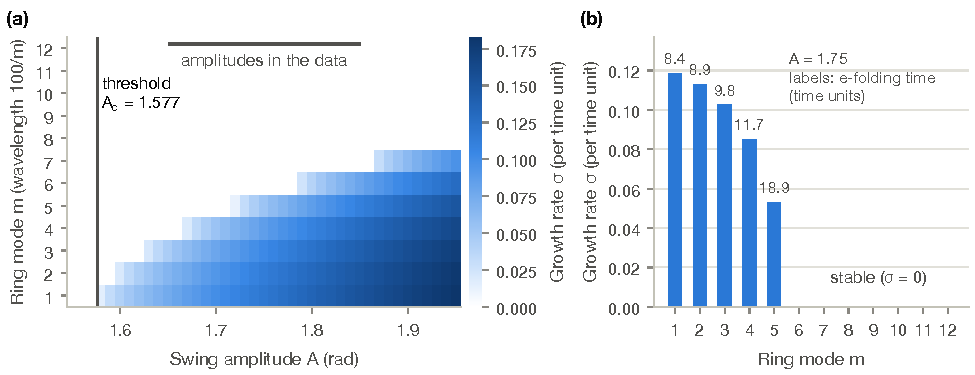
\includegraphics[width=\linewidth]{paper_fig1_spectrum.pdf}
  \caption{Floquet growth spectrum of the uniform swing, Eq.~(\ref{eq:hill}). (a)~Growth rate $\sigma_m$ of ring mode $m$ (wavelength $100/m$ pendulums) against the swing amplitude $A$; the swing becomes unstable at $A_c=1.577$, and the bar marks the amplitudes in the data. (b)~At $A=1.75$ only modes $m=1$--$5$ grow; the labels give the $e$-folding time of each mode.}
  \label{fig:spectrum}
\end{figure}

Figure~\ref{fig:spectrum} shows the resulting spectrum. The uniform swing becomes unstable at $A_c=1.577$, consistent with the vertical asymptote of the localization time near $A=1.59$ found numerically in Ref.~\cite{mittal2026jand}. As the amplitude increases, more long waves become unstable, but only a few do in the range used here: at $A=1.75$ only the five longest waves grow, with wavelengths of 100, 50, 33, 25 and 20 pendulums. The fastest grows by a factor of $e$ every 8.4 time units, so during the first 4.5 time units after release, the observation window of Ref.~\cite{mittal2026jand}, the perturbation grows by less than a factor of two.

Three expectations follow, and they guide everything below. First, since the growing modes are the longest waves of the ring, the eventual site should be a property of the whole ring rather than of a local neighborhood. Second, since so little growth occurs in the observation window, a predictor must essentially read the initial perturbation and project it onto the growing modes, rather than watch the hotspot form. Third, little else happens in time during that window: a small-amplitude estimate of the largest group velocity gives about half a pendulum per time unit, so a disturbance moves by only about two pendulums. Moreover, since the ring is released from rest, the initial angles $\theta_n(0)$ are its complete state, and everything observed later is a function of them.

\subsection{Simulation, labels and metrics}
\label{sec:pools}

Training some 750 networks requires far more simulated runs than Ref.~\cite{mittal2026jand} did, so we replaced its run-by-run \texttt{odeint} integration \cite{virtanen2020scipy} with a fourth-order Runge--Kutta scheme \cite{press1992numerical} that integrates thousands of runs at once (step $\Delta\tau=0.05$; samples every 0.5 time units, as before). On 1,000 test runs it gives exactly the same localization site and time as the simulation code of Ref.~\cite{mittal2026jand}, more than ten times faster. Since the simulation is deterministic, we store only the initial angles of each run and regenerate any model input from them. Models are trained on up to 100,000 runs, the first 60,000 matching the training budget of Ref.~\cite{mittal2026jand}; a validation pool of 20,000 runs serves for every model choice, and a test pool of 20,000 runs only for the numbers we report. The pools are generated with different random seeds, so no run appears in two of them, and inputs are standardized with statistics of the training pool alone. Sections~\ref{sec:physics} and \ref{sec:realchain} use further pools of 75,000 runs at fixed amplitudes and on rings of other sizes, and the runs of the main pools with their offsets rescaled, with labels searched up to $\tau=300$.

Following Ref.~\cite{mittal2026jand}, a run localizes at the first sample at which one site holds more than 10\% of the total energy, $\max_n E_n>0.1\,\Etot$, and its label is that site. We call this the \emph{first-crossing label} and, with the offsets above, use it for every comparison with v1, since these are the settings stated in Ref.~\cite{mittal2026jand} (Sec.~\ref{sec:repro}); Sec.~\ref{sec:target} introduces smoother labels and examines the choice of threshold. Distances are measured around the ring, $d(n,n')=\min(|n-n'|,\,N-|n-n'|)$. Accuracy within $\pm1$, the metric of Ref.~\cite{mittal2026jand}, was chosen there because the localized energy spans several pendulums, a point that Sec.~\ref{sec:target} bears out; it also partly rewards a convention, since in 19\% of test runs, which pendulum crosses first changes if the spring energy in Eq.~(\ref{eq:energy}) is split evenly between neighbors. We therefore also report the mean distance between predicted and true site, the accuracy within $\pm3$, and the share of runs more than 10 sites off, which we call far misses. The test pool resolves an accuracy to a standard error of 0.3\%.

\subsection{Predictors and protocol}
\label{sec:predictors}

We compare the networks with three physics baselines. The \emph{box-car} predictor of Ref.~\cite{mittal2026jand} picks the site where a moving average of the site energy peaks, with the width and the time of the snapshot chosen on the validation pool. The \emph{Floquet filter} needs no training at all: it evolves the mean-subtracted initial angles through the linearized dynamics for six swing periods, multiplying each ring mode by its response computed from $M_m(A)$ at the run's estimated amplitude, and picks the site where the result peaks. The \emph{linear ring filter} is the simplest trained model that respects the ring, a multinomial logistic regression whose score at each site is a circular convolution of the initial angles over the whole ring, with amplitude-dependent weights (200 parameters); it is convex, and we fit it to its global optimum with L-BFGS \cite{liu1989limited}. The network of Ref.~\cite{mittal2026jand}, v1, takes the site energies at $\tau=0,0.5,\dots,4.5$, each frame paired with the initial angles $\theta_n(0)$. Four convolutions extract features from each of the ten frames, a bidirectional long short-term memory (LSTM) layer combines the frames, and a dense layer feeds two outputs, the probability that the run localizes and a probability for each of the 100 sites; the network has 26.5 million parameters. Since its training code was not available for this study, we rebuilt it in PyTorch \cite{paszke2019pytorch} from Sec.~2.3 and the Appendix of Ref.~\cite{mittal2026jand} (Sec.~\ref{sec:repro} and Appendix~\ref{app:training}).

The study proceeded question by question. We first compared architectures, with v1's inputs, then the inputs, the loss and the optimizer, changing one choice at a time; finally we combined the best choices and removed them again one at a time to see which mattered. Inputs, losses and optimizers were compared in shorter screening runs with up to three training seeds (random initializations of the network), the final model with five. Every network was trained on one laptop (an Apple M3 Pro, mostly on its built-in GPU); training details are given in Appendix~\ref{app:training}.

% ===========================================================================
\section{Results}
\label{sec:results}

\subsection{What the growth spectrum explains}
\label{sec:physics}

Let us first return to the box-car smoothing of Ref.~\cite{mittal2026jand}, whose best width, 17 pendulums, was found empirically. A box-car of width $K$ first cancels the ring mode $m=N/K$; a wider box-car also suppresses longer waves, and a narrower one lets shorter ones through. The best width should therefore cancel the first stable mode, $m_c$, while canceling none of the growing ones, which gives $K^*=N/m_c$, or $100/6\approx17$ at $A=1.75$, where modes 1--5 grow. Figure~\ref{fig:physics}(a) shows that this prediction follows the best width measured at seven amplitudes, from just above threshold to $A=1.90$. The energetic clusters identified in Ref.~\cite{mittal2026jand} thus appear to be the growing long waves, seen through a low-pass filter.

\begin{figure}[t]
  \centering
  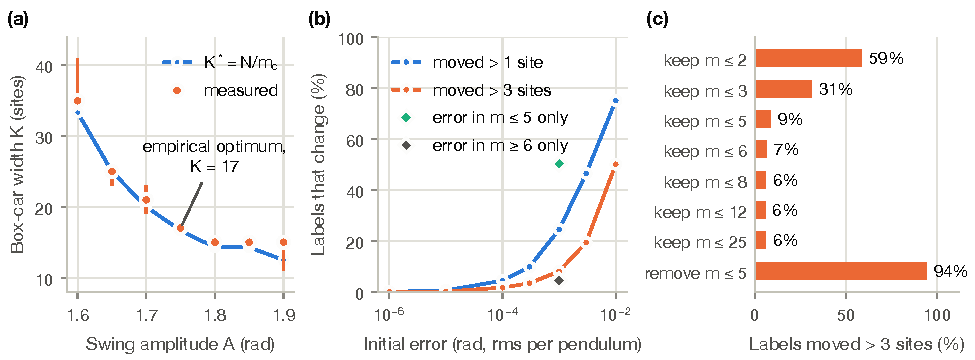
\includegraphics[width=\linewidth]{paper_fig2_physics.pdf}
  \caption{(a)~The best box-car width (dots, with 16--84\% bootstrap ranges; 2,000 runs per amplitude) follows the Floquet band edge $K^*=N/m_c$ (line), where $m_c$ is the first stable mode; the empirical optimum of Ref.~\cite{mittal2026jand} lies on it. (b)~Share of labels moved by more than one or three sites when white noise of the given size is added to the initial angles; diamonds give the share moved by more than one site when a $10^{-3}$~rad error is placed only in modes $m\le5$ or only in $m\ge6$. (c)~Share of labels moved by more than three sites when the initial perturbation keeps only the modes $m\le M$, or loses the modes $m\le5$.}
  \label{fig:physics}
\end{figure}

Since the localization process is noise-activated, one may ask next whether chaos limits how well it can be predicted. Figure~\ref{fig:physics}(b) shows that it does not. Perturbing the initial angles by $10^{-6}$~rad never changes the label, and neither does halving the integration step, so the label is a deterministic function of the initial state and the best possible accuracy is close to 100\%. What limits prediction is how precisely that state is known: an error of $10^{-3}$~rad on every pendulum moves a quarter of the labels by more than one site, and placed only in the five longest modes, it moves half of them. Conversely [Fig.~\ref{fig:physics}(c)], deleting every initial mode except the five longest keeps the site within $\pm3$ in 91\% of runs, whereas deleting those five makes the site random. The coarse answer thus lives in about ten numbers, the amplitudes and phases of the five growing modes, while local detail decides the last site or two.

The spectrum also sets the clock. To separate the growth rate from everything else that changes with the amplitude, we simulated runs at eight fixed amplitudes between 1.60 and 1.95, over which $\sigma_1$ rises from 0.042 to 0.183 and the number of growing modes from two to seven. The first pendulum goes over the top after a median of 120 time units at the lowest amplitude and 33 at the highest, yet this time multiplied by $\sigma_1$ stays between 5.0 and 6.0 [Fig.~\ref{fig:clock}(a)]. Localization thus takes 5--6 $e$-foldings of the fastest mode at any amplitude (median 5.75 over a pool spanning the whole interval), roughly what the growing modes need to rise from the size the offsets give them, about 0.002~rad each, to the 1.4~rad that carries a pendulum over the top, consistent with the picture of localization as a modulational instability followed by nonlinear focusing \cite{dauxois1993energy,daumont1997modulational}. The amplitudes of Ref.~\cite{mittal2026jand} are best described as growth rates of 0.075--0.153.

The offsets are the release scatter, part of the physics rather than noise: since the uniform swing is an exact solution of Eq.~(\ref{eq:eom}), without them nothing would localize. Scaling the offsets of the same runs by a factor $s$ between 1/8 and 4 should shift the localization time by $\ln(1/s)/\sigma_1$, and the measured delays follow this with a slope of 1.10 [Fig.~\ref{fig:clock}(b)], the effective growth being slightly slower than that of the fastest mode, as we find again for sensor noise in Sec.~\ref{sec:realchain}. The size of the offsets also moves the site: between the stated offsets and an eighth of them, it stays in place in only 37\% of runs. With smaller offsets the growing modes need longer to rise, while the modes that do not grow keep their size, since the Floquet multipliers of a stable mode of Eq.~(\ref{eq:hill}) lie on the unit circle \cite{magnus1966hill}, so that their local detail weighs less when the hump forms. Linear theory reaches correspondingly further. The Floquet filter places 52\% of runs within $\pm1$ of the first pendulum over the top at four times the offsets, 73\% at the stated ones and 87\% at an eighth, and across amplitudes its accuracy falls as the offsets grow relative to the distance above threshold, $\eta_{\max}/(A-A_c)$, down to 17\% at $A=1.60$, where this ratio is about one [Fig.~\ref{fig:clock}(c)]. Close to the threshold, where only a few modes grow at similar rates, it stays below 65\% even with small offsets. A network trained on each condition, by contrast, places at least 98.4\% of runs within $\pm1$, learning what linear theory misses.

\begin{figure}[t]
  \centering
  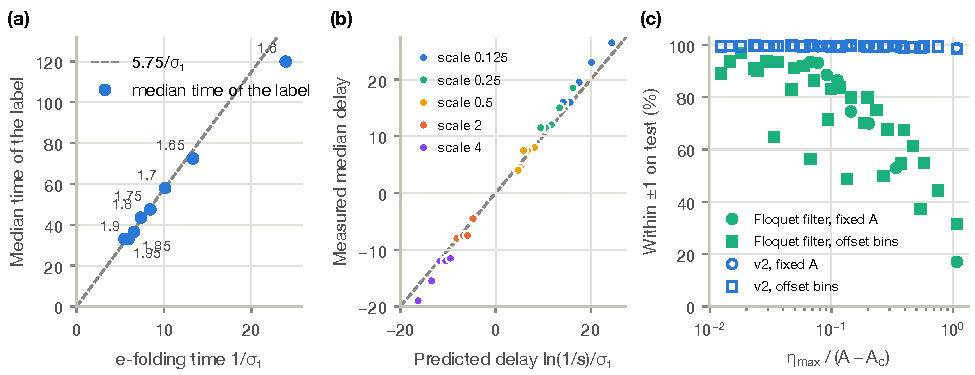
\includegraphics[width=\linewidth]{paper_fig_clock.pdf}
  \caption{The growth spectrum sets the clock (test pools). (a)~Median time at which the first pendulum goes over the top, at eight fixed amplitudes (labels), against the $e$-folding time of the fastest mode; the line is $5.75/\sigma_1$. (b)~Median delay of that time when the offsets of the same runs are scaled by $s$, against the prediction $\ln(1/s)/\sigma_1$, in five amplitude bins. (c)~Accuracy within $\pm1$ of the Floquet filter (filled) and of v2 trained on each condition (open; event-timed hump label of Sec.~\ref{sec:target}, three seeds) against the size of the offsets relative to the distance above threshold, for fixed amplitudes and for amplitude bins of the rescaled pools.}
  \label{fig:clock}
\end{figure}

The physics alone already gets far (Table~\ref{tab:headline}). The best box-car reaches a mean distance of 5.07 sites, close to the 5.4 reported in Ref.~\cite{mittal2026jand}. The Floquet filter, which simply grows the measured initial perturbation and has no trained parameters, matches the mean distance of the rebuilt v1 (3.12 against 3.14), although it is less often within $\pm1$. The 200-parameter linear ring filter beats the rebuilt v1 on every metric. These baselines set the bar that any network has to clear.

\begin{table}[t]
  \centering
  \caption{Predictors on the 20,000-run test pool (first-crossing label; mean over the seeds in brackets, $\pm$ standard deviation). Distances in sites, accuracies in \%. The scores in the first row are quoted from Ref.~\cite{mittal2026jand}, which does not state whether its 1.44 wraps around the ring (without wrapping, v2 scores 2.43); they appear to have been obtained with a lower threshold and smaller offsets (Sec.~\ref{sec:repro}).}
  \label{tab:headline}
  \small
  \setlength{\tabcolsep}{4pt}
  \begin{tabular}{@{}lrrrrrr@{}}
    \toprule
    Predictor [seeds] & Parameters & Mean dist. & Exact & $\pm1$ & $\pm3$ & $>10$ off \\
    \midrule
    v1, as published \cite{mittal2026jand} & 26.5M & 1.44 & & 94.4 & & \\
    v1, rebuilt [2] & 26.5M & $3.14\pm0.19$ & 22.5 & $60.4\pm1.9$ & 90.3 & 5.7 \\
    Box-car, $K=17$, best snapshot & 0 & 5.07 & 12.9 & 38.0 & 71.1 & 9.0 \\
    Floquet filter & 0 & 3.12 & 20.7 & 52.0 & 87.3 & 4.6 \\
    Linear ring filter & 200 & 2.17 & 27.3 & 67.4 & 95.3 & 3.1 \\
    \textbf{v2 [5]} & \textbf{22,786} & $\mathbf{1.49\pm0.03}$ & \textbf{27.7} & $\mathbf{77.2\pm0.5}$ & \textbf{97.3} & \textbf{1.5} \\
    \bottomrule
  \end{tabular}
\end{table}

\subsection{A network built around the ring}
\label{sec:arch}

\begin{figure}[t]
  \centering
  % Schematic of the v1 and v2 networks (TikZ, plain pdflatex).
% Used as \begin{figure}[t]\centering% Schematic of the v1 and v2 networks (TikZ, plain pdflatex).
% Used as \begin{figure}[t]\centering% Schematic of the v1 and v2 networks (TikZ, plain pdflatex).
% Used as \begin{figure}[t]\centering\input{fig_schematic}\caption{...}\end{figure}.
% Needs in the preamble: \usepackage{tikz}
%                        \usetikzlibrary{arrows.meta,calc}
% Parameter counts from sgloc/models.py (V1CnnBiLstm; RingNet with the final ARCH and a time head):
%   v1 26,499,205 = convs 129,696 + BiLSTM 26,346,496 (input weights 26,214,400) + dense 16,448 + heads 6,565
%   v2     22,786 = 7 convs 19,616 + per-site head 3,137 + time head 33
% Under the BiLSTM the figure gives its input weights, 26.2M (98.9%), the number quoted in the text.
\begin{tikzpicture}[x=1cm, y=1cm, font=\footnotesize, line join=round,
  arr/.style={-{Stealth[length=3.4pt, width=3pt]}, line width=0.6pt, draw=sgInk},
  softarr/.style={-{Stealth[length=2.6pt, width=2.4pt]}, line width=0.5pt},
  box1/.style={draw=sgOneLine, fill=sgOneFill, line width=0.6pt, rounded corners=1.2pt},
  box2/.style={draw=sgTwoLine, fill=sgTwoFill, line width=0.6pt, rounded corners=1.2pt},
  slab1/.style={box1, minimum width=0.56cm, minimum height=1.2cm, anchor=south west, inner sep=0pt, font=\scriptsize},
  slab2/.style={box2, minimum width=0.42cm, minimum height=1.2cm, anchor=south west, inner sep=0pt, font=\scriptsize},
  note/.style={font=\scriptsize, text=sgInkTwo, align=center, inner sep=0.5pt},
  param/.style={font=\scriptsize, text=sgMuted, inner sep=0.5pt, anchor=base},
  rowlabel/.style={font=\footnotesize\bfseries, text=sgInk, anchor=base west, inner sep=0pt},
  tag/.style={font=\scriptsize, text=white, fill=sgInkTwo, rounded corners=1.2pt, inner sep=1.6pt},
]
\definecolor{sgOneLine}{HTML}{B4602E}
\definecolor{sgOneFill}{HTML}{FBE9DC}
\definecolor{sgOneMid}{HTML}{F1C3A3}
\definecolor{sgTwoLine}{HTML}{2F67A6}
\definecolor{sgTwoFill}{HTML}{E0EBF7}
\definecolor{sgTwoMid}{HTML}{B3CDEB}
\definecolor{sgInk}{HTML}{2B2B2A}
\definecolor{sgInkTwo}{HTML}{52514E}
\definecolor{sgMuted}{HTML}{7A7973}
\definecolor{sgDot}{HTML}{C9C8C1}

% =====================================================================
% (a) v1: CNN-BiLSTM
% =====================================================================
\begin{scope}
\node[rowlabel] at (0,1.25) {(a) v1: CNN-BiLSTM};

% input: 10 frames of 100 sites, two channels each
\foreach \j in {9,...,1}
  \draw[box1, line width=0.4pt] ($(0,-0.46)+(0.05*\j,0.05*\j)$) rectangle +(1.45,0.46);
\draw[box1] (0,-0.46) rectangle (1.45,0);
\begin{scope}
  \clip[rounded corners=1.2pt] (0,-0.46) rectangle (1.45,0);
  \fill[sgOneMid] (0,-0.23) rectangle (1.45,0);
\end{scope}
\draw[box1, fill=none] (0,-0.46) rectangle (1.45,0);
\draw[sgOneLine, line width=0.4pt] (0,-0.23) -- (1.45,-0.23);
\node[note, anchor=north] at (0.95,-0.62) {$E_n(\tau)$, $\theta_n(0)$\\10 frames};

% per-frame part: four convolutions, then flatten
\draw[sgMuted, line width=0.5pt, dash pattern=on 2pt off 1.5pt, rounded corners=3pt] (2.3,-0.74) rectangle (5.84,0.78);
\node[font=\scriptsize, text=sgInkTwo, fill=white, inner sep=1.5pt, anchor=west] at (2.5,0.78) {each frame separately};
\draw[arr] (1.97,0) -- (2.42,0);
\foreach \f [count=\k from 0] in {32,64,128,256}
  \node[slab1] at (2.48+0.62*\k,-0.6) {\f};
\draw[arr] (4.94,0) -- (5.3,0);
\fill[sgOneFill] (5.36,-0.6) rectangle (5.52,0.6);
\foreach \k in {1,...,11} \draw[sgOneMid, line width=0.3pt] (5.36,-0.6+0.1*\k) -- (5.52,-0.6+0.1*\k);
\draw[sgOneLine, line width=0.6pt] (5.36,-0.6) rectangle (5.52,0.6);
\node[note, anchor=north] at (3.69,-0.84) {filters, kernel 3\\zero padding};
\node[note, anchor=north] at (5.44,-0.84) {flatten\\25,600};

% bidirectional LSTM over the 10 frames
\draw[arr] (5.84,0) -- (6.26,0);
\node[box1, minimum width=1.85cm, minimum height=1.2cm, anchor=west] (lstm) at (6.32,0) {};
\node[font=\footnotesize, anchor=base] at (7.245,0.25) {BiLSTM};
\node[note, anchor=base] at (7.245,0.0) {128 + 128};
\foreach \k in {0,...,9} \fill[sgOneLine] (6.62+0.139*\k,-0.29) circle (0.028);
\draw[softarr, sgOneLine] (6.57,-0.17) -- (7.92,-0.17);
\draw[softarr, sgOneLine] (7.92,-0.42) -- (6.57,-0.42);
\node[tag, anchor=south] (tagA) at (7.245,0.84) {space and time meet};
\draw[arr, draw=sgInkTwo] (tagA.south) -- (7.245,0.63);

% dense layer and the two heads
\draw[arr] (8.17,0) -- (8.5,0);
\node[box1, minimum width=0.95cm, minimum height=0.84cm, anchor=west, align=center, inner sep=0.5pt, font=\scriptsize]
  (dense) at (8.55,0) {dense\\64};
\draw[arr] (9.5,0) -- (9.68,0) |- (9.86,0.4);
\draw[arr] (9.68,0) |- (9.86,-0.4);
\foreach \i in {0,...,19} {
  \pgfmathtruncatemacro{\p}{round(90*exp(-(\i-12)^2/3.5))}
  \fill[sgOneLine!\p!sgOneFill] (9.92+0.14*\i,0.23) rectangle +(0.14,0.34);
}
\draw[sgOneLine, line width=0.6pt] (9.92,0.23) rectangle (12.72,0.57);
\node[note, anchor=south] at (11.32,0.62) {softmax over 100 sites};
\node[box1, minimum width=2.8cm, minimum height=0.34cm, anchor=west, inner sep=0.5pt, font=\scriptsize]
  at (9.92,-0.4) {localizes? (sigmoid)};

% what a convolutional feature sees
\begin{scope}[shift={(14.55,0.05)}]
  \draw[sgOneMid, line width=4pt] (73.8:0.58) arc[start angle=73.8, end angle=106.2, radius=0.58];
  \foreach \i in {0,...,99} \fill[sgDot] (3.6*\i:0.58) circle (0.012);
  \foreach \i in {-4,...,4} \fill[sgOneLine] (90+3.6*\i:0.58) circle (0.017);
  \fill[sgOneLine] (90:0.58) circle (0.04);
\end{scope}
\node[note, anchor=north] at (14.55,-0.7) {each conv feature\\sees 9 sites};

% where the parameters sit
\node[param, anchor=base west, font=\scriptsize\itshape] at (0,-1.85) {parameters};
\node[param] at (3.69,-1.85) {0.13M};
\node[param, text=sgOneLine] at (7.245,-1.85) {\textbf{26.2M} (99\%)};
\node[param, text=sgOneLine] at (7.245,-2.17) {input weights};
\node[param] at (9.025,-1.85) {16k};
\node[param] at (11.32,-1.85) {6.6k};
\node[param, text=sgInk] at (14.55,-1.85) {total 26,499,205};
\end{scope}

% =====================================================================
% (b) v2: ring network
% =====================================================================
\begin{scope}[yshift=-3.95cm]
\node[rowlabel] at (0,1.25) {(b) v2: ring network};

% input: the 10 angle frames stacked as channels of one signal on the ring
\foreach \k in {0,...,9} {
  \ifodd\k \def\sgStripe{sgTwoMid}\else\def\sgStripe{sgTwoFill}\fi
  \fill[\sgStripe] (0,-0.5+0.1*\k) rectangle (1.9,-0.4+0.1*\k);
}
\draw[sgTwoLine, line width=0.6pt] (0,-0.5) rectangle (1.9,0.5);
\node[note, anchor=north] at (0.95,-0.62) {$\theta_n(\tau)$, 10 frames\\as channels};

% seven circular convolutions; the numbers are the dilations
\draw[arr] (1.97,0) -- (2.42,0);
\foreach \d [count=\k from 0] in {1,2,4,8,16,32,1}
  \node[slab2] at (2.48+0.5*\k,-0.6) {\d};
\node[tag, anchor=west] (tagB) at (3.3,0.9) {space and time meet};
\draw[arr, draw=sgInkTwo] (tagB.west) -| (2.69,0.63);
\node[note, anchor=north] at (4.2,-0.72) {dilation, kernel 3\\32 channels, circular};

% per-site head and time head
\draw[arr] (5.9,0) -- (6.1,0) |- (6.3,0.4);
\draw[arr] (6.1,0) |- (6.3,-0.4);
\node[box2, minimum width=3.0cm, minimum height=0.6cm, anchor=west, align=center, inner sep=0.5pt, font=\scriptsize]
  at (6.35,0.4) {per-site head\\conv 3 + 1$\times$1};
\node[box2, minimum width=3.0cm, minimum height=0.6cm, anchor=west, align=center, inner sep=0.5pt, font=\scriptsize]
  at (6.35,-0.4) {ring average\\linear};
\draw[arr] (9.35,0.4) -- (9.86,0.4);
\draw[arr] (9.35,-0.4) -- (9.86,-0.4);
\foreach \i in {0,...,19} {
  \pgfmathtruncatemacro{\p}{round(90*exp(-(\i-12)^2/3.5))}
  \fill[sgTwoLine!\p!sgTwoFill] (9.92+0.14*\i,0.23) rectangle +(0.14,0.34);
}
\draw[sgTwoLine, line width=0.6pt] (9.92,0.23) rectangle (12.72,0.57);
\node[note, anchor=south] at (11.32,0.62) {$p_n$, softmax over the ring};
\node[box2, minimum width=2.8cm, minimum height=0.34cm, anchor=west, inner sep=0.5pt, font=\scriptsize]
  at (9.92,-0.4) {$\ln\tau_{\mathrm{loc}}$};

% what one site sees
\begin{scope}[shift={(14.55,0.05)}]
  \draw[sgTwoMid, line width=4pt] (0,0) circle (0.58);
  \foreach \i in {0,...,99} \fill[sgTwoLine] (3.6*\i:0.58) circle (0.017);
  \fill[sgTwoLine] (90:0.58) circle (0.04);
\end{scope}
\node[note, anchor=north] at (14.55,-0.7) {each site sees\\129 sites $>$ 100};

% where the parameters sit
\node[param, anchor=base west, font=\scriptsize\itshape] at (0,-1.85) {parameters};
\node[param] at (4.2,-1.85) {19.6k};
\node[param] at (7.85,-1.85) {3.1k + 33};
\node[param, text=sgInk] at (14.55,-1.85) {total 22,786};
\end{scope}
\end{tikzpicture}
\caption{...}\end{figure}.
% Needs in the preamble: \usepackage{tikz}
%                        \usetikzlibrary{arrows.meta,calc}
% Parameter counts from sgloc/models.py (V1CnnBiLstm; RingNet with the final ARCH and a time head):
%   v1 26,499,205 = convs 129,696 + BiLSTM 26,346,496 (input weights 26,214,400) + dense 16,448 + heads 6,565
%   v2     22,786 = 7 convs 19,616 + per-site head 3,137 + time head 33
% Under the BiLSTM the figure gives its input weights, 26.2M (98.9%), the number quoted in the text.
\begin{tikzpicture}[x=1cm, y=1cm, font=\footnotesize, line join=round,
  arr/.style={-{Stealth[length=3.4pt, width=3pt]}, line width=0.6pt, draw=sgInk},
  softarr/.style={-{Stealth[length=2.6pt, width=2.4pt]}, line width=0.5pt},
  box1/.style={draw=sgOneLine, fill=sgOneFill, line width=0.6pt, rounded corners=1.2pt},
  box2/.style={draw=sgTwoLine, fill=sgTwoFill, line width=0.6pt, rounded corners=1.2pt},
  slab1/.style={box1, minimum width=0.56cm, minimum height=1.2cm, anchor=south west, inner sep=0pt, font=\scriptsize},
  slab2/.style={box2, minimum width=0.42cm, minimum height=1.2cm, anchor=south west, inner sep=0pt, font=\scriptsize},
  note/.style={font=\scriptsize, text=sgInkTwo, align=center, inner sep=0.5pt},
  param/.style={font=\scriptsize, text=sgMuted, inner sep=0.5pt, anchor=base},
  rowlabel/.style={font=\footnotesize\bfseries, text=sgInk, anchor=base west, inner sep=0pt},
  tag/.style={font=\scriptsize, text=white, fill=sgInkTwo, rounded corners=1.2pt, inner sep=1.6pt},
]
\definecolor{sgOneLine}{HTML}{B4602E}
\definecolor{sgOneFill}{HTML}{FBE9DC}
\definecolor{sgOneMid}{HTML}{F1C3A3}
\definecolor{sgTwoLine}{HTML}{2F67A6}
\definecolor{sgTwoFill}{HTML}{E0EBF7}
\definecolor{sgTwoMid}{HTML}{B3CDEB}
\definecolor{sgInk}{HTML}{2B2B2A}
\definecolor{sgInkTwo}{HTML}{52514E}
\definecolor{sgMuted}{HTML}{7A7973}
\definecolor{sgDot}{HTML}{C9C8C1}

% =====================================================================
% (a) v1: CNN-BiLSTM
% =====================================================================
\begin{scope}
\node[rowlabel] at (0,1.25) {(a) v1: CNN-BiLSTM};

% input: 10 frames of 100 sites, two channels each
\foreach \j in {9,...,1}
  \draw[box1, line width=0.4pt] ($(0,-0.46)+(0.05*\j,0.05*\j)$) rectangle +(1.45,0.46);
\draw[box1] (0,-0.46) rectangle (1.45,0);
\begin{scope}
  \clip[rounded corners=1.2pt] (0,-0.46) rectangle (1.45,0);
  \fill[sgOneMid] (0,-0.23) rectangle (1.45,0);
\end{scope}
\draw[box1, fill=none] (0,-0.46) rectangle (1.45,0);
\draw[sgOneLine, line width=0.4pt] (0,-0.23) -- (1.45,-0.23);
\node[note, anchor=north] at (0.95,-0.62) {$E_n(\tau)$, $\theta_n(0)$\\10 frames};

% per-frame part: four convolutions, then flatten
\draw[sgMuted, line width=0.5pt, dash pattern=on 2pt off 1.5pt, rounded corners=3pt] (2.3,-0.74) rectangle (5.84,0.78);
\node[font=\scriptsize, text=sgInkTwo, fill=white, inner sep=1.5pt, anchor=west] at (2.5,0.78) {each frame separately};
\draw[arr] (1.97,0) -- (2.42,0);
\foreach \f [count=\k from 0] in {32,64,128,256}
  \node[slab1] at (2.48+0.62*\k,-0.6) {\f};
\draw[arr] (4.94,0) -- (5.3,0);
\fill[sgOneFill] (5.36,-0.6) rectangle (5.52,0.6);
\foreach \k in {1,...,11} \draw[sgOneMid, line width=0.3pt] (5.36,-0.6+0.1*\k) -- (5.52,-0.6+0.1*\k);
\draw[sgOneLine, line width=0.6pt] (5.36,-0.6) rectangle (5.52,0.6);
\node[note, anchor=north] at (3.69,-0.84) {filters, kernel 3\\zero padding};
\node[note, anchor=north] at (5.44,-0.84) {flatten\\25,600};

% bidirectional LSTM over the 10 frames
\draw[arr] (5.84,0) -- (6.26,0);
\node[box1, minimum width=1.85cm, minimum height=1.2cm, anchor=west] (lstm) at (6.32,0) {};
\node[font=\footnotesize, anchor=base] at (7.245,0.25) {BiLSTM};
\node[note, anchor=base] at (7.245,0.0) {128 + 128};
\foreach \k in {0,...,9} \fill[sgOneLine] (6.62+0.139*\k,-0.29) circle (0.028);
\draw[softarr, sgOneLine] (6.57,-0.17) -- (7.92,-0.17);
\draw[softarr, sgOneLine] (7.92,-0.42) -- (6.57,-0.42);
\node[tag, anchor=south] (tagA) at (7.245,0.84) {space and time meet};
\draw[arr, draw=sgInkTwo] (tagA.south) -- (7.245,0.63);

% dense layer and the two heads
\draw[arr] (8.17,0) -- (8.5,0);
\node[box1, minimum width=0.95cm, minimum height=0.84cm, anchor=west, align=center, inner sep=0.5pt, font=\scriptsize]
  (dense) at (8.55,0) {dense\\64};
\draw[arr] (9.5,0) -- (9.68,0) |- (9.86,0.4);
\draw[arr] (9.68,0) |- (9.86,-0.4);
\foreach \i in {0,...,19} {
  \pgfmathtruncatemacro{\p}{round(90*exp(-(\i-12)^2/3.5))}
  \fill[sgOneLine!\p!sgOneFill] (9.92+0.14*\i,0.23) rectangle +(0.14,0.34);
}
\draw[sgOneLine, line width=0.6pt] (9.92,0.23) rectangle (12.72,0.57);
\node[note, anchor=south] at (11.32,0.62) {softmax over 100 sites};
\node[box1, minimum width=2.8cm, minimum height=0.34cm, anchor=west, inner sep=0.5pt, font=\scriptsize]
  at (9.92,-0.4) {localizes? (sigmoid)};

% what a convolutional feature sees
\begin{scope}[shift={(14.55,0.05)}]
  \draw[sgOneMid, line width=4pt] (73.8:0.58) arc[start angle=73.8, end angle=106.2, radius=0.58];
  \foreach \i in {0,...,99} \fill[sgDot] (3.6*\i:0.58) circle (0.012);
  \foreach \i in {-4,...,4} \fill[sgOneLine] (90+3.6*\i:0.58) circle (0.017);
  \fill[sgOneLine] (90:0.58) circle (0.04);
\end{scope}
\node[note, anchor=north] at (14.55,-0.7) {each conv feature\\sees 9 sites};

% where the parameters sit
\node[param, anchor=base west, font=\scriptsize\itshape] at (0,-1.85) {parameters};
\node[param] at (3.69,-1.85) {0.13M};
\node[param, text=sgOneLine] at (7.245,-1.85) {\textbf{26.2M} (99\%)};
\node[param, text=sgOneLine] at (7.245,-2.17) {input weights};
\node[param] at (9.025,-1.85) {16k};
\node[param] at (11.32,-1.85) {6.6k};
\node[param, text=sgInk] at (14.55,-1.85) {total 26,499,205};
\end{scope}

% =====================================================================
% (b) v2: ring network
% =====================================================================
\begin{scope}[yshift=-3.95cm]
\node[rowlabel] at (0,1.25) {(b) v2: ring network};

% input: the 10 angle frames stacked as channels of one signal on the ring
\foreach \k in {0,...,9} {
  \ifodd\k \def\sgStripe{sgTwoMid}\else\def\sgStripe{sgTwoFill}\fi
  \fill[\sgStripe] (0,-0.5+0.1*\k) rectangle (1.9,-0.4+0.1*\k);
}
\draw[sgTwoLine, line width=0.6pt] (0,-0.5) rectangle (1.9,0.5);
\node[note, anchor=north] at (0.95,-0.62) {$\theta_n(\tau)$, 10 frames\\as channels};

% seven circular convolutions; the numbers are the dilations
\draw[arr] (1.97,0) -- (2.42,0);
\foreach \d [count=\k from 0] in {1,2,4,8,16,32,1}
  \node[slab2] at (2.48+0.5*\k,-0.6) {\d};
\node[tag, anchor=west] (tagB) at (3.3,0.9) {space and time meet};
\draw[arr, draw=sgInkTwo] (tagB.west) -| (2.69,0.63);
\node[note, anchor=north] at (4.2,-0.72) {dilation, kernel 3\\32 channels, circular};

% per-site head and time head
\draw[arr] (5.9,0) -- (6.1,0) |- (6.3,0.4);
\draw[arr] (6.1,0) |- (6.3,-0.4);
\node[box2, minimum width=3.0cm, minimum height=0.6cm, anchor=west, align=center, inner sep=0.5pt, font=\scriptsize]
  at (6.35,0.4) {per-site head\\conv 3 + 1$\times$1};
\node[box2, minimum width=3.0cm, minimum height=0.6cm, anchor=west, align=center, inner sep=0.5pt, font=\scriptsize]
  at (6.35,-0.4) {ring average\\linear};
\draw[arr] (9.35,0.4) -- (9.86,0.4);
\draw[arr] (9.35,-0.4) -- (9.86,-0.4);
\foreach \i in {0,...,19} {
  \pgfmathtruncatemacro{\p}{round(90*exp(-(\i-12)^2/3.5))}
  \fill[sgTwoLine!\p!sgTwoFill] (9.92+0.14*\i,0.23) rectangle +(0.14,0.34);
}
\draw[sgTwoLine, line width=0.6pt] (9.92,0.23) rectangle (12.72,0.57);
\node[note, anchor=south] at (11.32,0.62) {$p_n$, softmax over the ring};
\node[box2, minimum width=2.8cm, minimum height=0.34cm, anchor=west, inner sep=0.5pt, font=\scriptsize]
  at (9.92,-0.4) {$\ln\tau_{\mathrm{loc}}$};

% what one site sees
\begin{scope}[shift={(14.55,0.05)}]
  \draw[sgTwoMid, line width=4pt] (0,0) circle (0.58);
  \foreach \i in {0,...,99} \fill[sgTwoLine] (3.6*\i:0.58) circle (0.017);
  \fill[sgTwoLine] (90:0.58) circle (0.04);
\end{scope}
\node[note, anchor=north] at (14.55,-0.7) {each site sees\\129 sites $>$ 100};

% where the parameters sit
\node[param, anchor=base west, font=\scriptsize\itshape] at (0,-1.85) {parameters};
\node[param] at (4.2,-1.85) {19.6k};
\node[param] at (7.85,-1.85) {3.1k + 33};
\node[param, text=sgInk] at (14.55,-1.85) {total 22,786};
\end{scope}
\end{tikzpicture}
\caption{...}\end{figure}.
% Needs in the preamble: \usepackage{tikz}
%                        \usetikzlibrary{arrows.meta,calc}
% Parameter counts from sgloc/models.py (V1CnnBiLstm; RingNet with the final ARCH and a time head):
%   v1 26,499,205 = convs 129,696 + BiLSTM 26,346,496 (input weights 26,214,400) + dense 16,448 + heads 6,565
%   v2     22,786 = 7 convs 19,616 + per-site head 3,137 + time head 33
% Under the BiLSTM the figure gives its input weights, 26.2M (98.9%), the number quoted in the text.
\begin{tikzpicture}[x=1cm, y=1cm, font=\footnotesize, line join=round,
  arr/.style={-{Stealth[length=3.4pt, width=3pt]}, line width=0.6pt, draw=sgInk},
  softarr/.style={-{Stealth[length=2.6pt, width=2.4pt]}, line width=0.5pt},
  box1/.style={draw=sgOneLine, fill=sgOneFill, line width=0.6pt, rounded corners=1.2pt},
  box2/.style={draw=sgTwoLine, fill=sgTwoFill, line width=0.6pt, rounded corners=1.2pt},
  slab1/.style={box1, minimum width=0.56cm, minimum height=1.2cm, anchor=south west, inner sep=0pt, font=\scriptsize},
  slab2/.style={box2, minimum width=0.42cm, minimum height=1.2cm, anchor=south west, inner sep=0pt, font=\scriptsize},
  note/.style={font=\scriptsize, text=sgInkTwo, align=center, inner sep=0.5pt},
  param/.style={font=\scriptsize, text=sgMuted, inner sep=0.5pt, anchor=base},
  rowlabel/.style={font=\footnotesize\bfseries, text=sgInk, anchor=base west, inner sep=0pt},
  tag/.style={font=\scriptsize, text=white, fill=sgInkTwo, rounded corners=1.2pt, inner sep=1.6pt},
]
\definecolor{sgOneLine}{HTML}{B4602E}
\definecolor{sgOneFill}{HTML}{FBE9DC}
\definecolor{sgOneMid}{HTML}{F1C3A3}
\definecolor{sgTwoLine}{HTML}{2F67A6}
\definecolor{sgTwoFill}{HTML}{E0EBF7}
\definecolor{sgTwoMid}{HTML}{B3CDEB}
\definecolor{sgInk}{HTML}{2B2B2A}
\definecolor{sgInkTwo}{HTML}{52514E}
\definecolor{sgMuted}{HTML}{7A7973}
\definecolor{sgDot}{HTML}{C9C8C1}

% =====================================================================
% (a) v1: CNN-BiLSTM
% =====================================================================
\begin{scope}
\node[rowlabel] at (0,1.25) {(a) v1: CNN-BiLSTM};

% input: 10 frames of 100 sites, two channels each
\foreach \j in {9,...,1}
  \draw[box1, line width=0.4pt] ($(0,-0.46)+(0.05*\j,0.05*\j)$) rectangle +(1.45,0.46);
\draw[box1] (0,-0.46) rectangle (1.45,0);
\begin{scope}
  \clip[rounded corners=1.2pt] (0,-0.46) rectangle (1.45,0);
  \fill[sgOneMid] (0,-0.23) rectangle (1.45,0);
\end{scope}
\draw[box1, fill=none] (0,-0.46) rectangle (1.45,0);
\draw[sgOneLine, line width=0.4pt] (0,-0.23) -- (1.45,-0.23);
\node[note, anchor=north] at (0.95,-0.62) {$E_n(\tau)$, $\theta_n(0)$\\10 frames};

% per-frame part: four convolutions, then flatten
\draw[sgMuted, line width=0.5pt, dash pattern=on 2pt off 1.5pt, rounded corners=3pt] (2.3,-0.74) rectangle (5.84,0.78);
\node[font=\scriptsize, text=sgInkTwo, fill=white, inner sep=1.5pt, anchor=west] at (2.5,0.78) {each frame separately};
\draw[arr] (1.97,0) -- (2.42,0);
\foreach \f [count=\k from 0] in {32,64,128,256}
  \node[slab1] at (2.48+0.62*\k,-0.6) {\f};
\draw[arr] (4.94,0) -- (5.3,0);
\fill[sgOneFill] (5.36,-0.6) rectangle (5.52,0.6);
\foreach \k in {1,...,11} \draw[sgOneMid, line width=0.3pt] (5.36,-0.6+0.1*\k) -- (5.52,-0.6+0.1*\k);
\draw[sgOneLine, line width=0.6pt] (5.36,-0.6) rectangle (5.52,0.6);
\node[note, anchor=north] at (3.69,-0.84) {filters, kernel 3\\zero padding};
\node[note, anchor=north] at (5.44,-0.84) {flatten\\25,600};

% bidirectional LSTM over the 10 frames
\draw[arr] (5.84,0) -- (6.26,0);
\node[box1, minimum width=1.85cm, minimum height=1.2cm, anchor=west] (lstm) at (6.32,0) {};
\node[font=\footnotesize, anchor=base] at (7.245,0.25) {BiLSTM};
\node[note, anchor=base] at (7.245,0.0) {128 + 128};
\foreach \k in {0,...,9} \fill[sgOneLine] (6.62+0.139*\k,-0.29) circle (0.028);
\draw[softarr, sgOneLine] (6.57,-0.17) -- (7.92,-0.17);
\draw[softarr, sgOneLine] (7.92,-0.42) -- (6.57,-0.42);
\node[tag, anchor=south] (tagA) at (7.245,0.84) {space and time meet};
\draw[arr, draw=sgInkTwo] (tagA.south) -- (7.245,0.63);

% dense layer and the two heads
\draw[arr] (8.17,0) -- (8.5,0);
\node[box1, minimum width=0.95cm, minimum height=0.84cm, anchor=west, align=center, inner sep=0.5pt, font=\scriptsize]
  (dense) at (8.55,0) {dense\\64};
\draw[arr] (9.5,0) -- (9.68,0) |- (9.86,0.4);
\draw[arr] (9.68,0) |- (9.86,-0.4);
\foreach \i in {0,...,19} {
  \pgfmathtruncatemacro{\p}{round(90*exp(-(\i-12)^2/3.5))}
  \fill[sgOneLine!\p!sgOneFill] (9.92+0.14*\i,0.23) rectangle +(0.14,0.34);
}
\draw[sgOneLine, line width=0.6pt] (9.92,0.23) rectangle (12.72,0.57);
\node[note, anchor=south] at (11.32,0.62) {softmax over 100 sites};
\node[box1, minimum width=2.8cm, minimum height=0.34cm, anchor=west, inner sep=0.5pt, font=\scriptsize]
  at (9.92,-0.4) {localizes? (sigmoid)};

% what a convolutional feature sees
\begin{scope}[shift={(14.55,0.05)}]
  \draw[sgOneMid, line width=4pt] (73.8:0.58) arc[start angle=73.8, end angle=106.2, radius=0.58];
  \foreach \i in {0,...,99} \fill[sgDot] (3.6*\i:0.58) circle (0.012);
  \foreach \i in {-4,...,4} \fill[sgOneLine] (90+3.6*\i:0.58) circle (0.017);
  \fill[sgOneLine] (90:0.58) circle (0.04);
\end{scope}
\node[note, anchor=north] at (14.55,-0.7) {each conv feature\\sees 9 sites};

% where the parameters sit
\node[param, anchor=base west, font=\scriptsize\itshape] at (0,-1.85) {parameters};
\node[param] at (3.69,-1.85) {0.13M};
\node[param, text=sgOneLine] at (7.245,-1.85) {\textbf{26.2M} (99\%)};
\node[param, text=sgOneLine] at (7.245,-2.17) {input weights};
\node[param] at (9.025,-1.85) {16k};
\node[param] at (11.32,-1.85) {6.6k};
\node[param, text=sgInk] at (14.55,-1.85) {total 26,499,205};
\end{scope}

% =====================================================================
% (b) v2: ring network
% =====================================================================
\begin{scope}[yshift=-3.95cm]
\node[rowlabel] at (0,1.25) {(b) v2: ring network};

% input: the 10 angle frames stacked as channels of one signal on the ring
\foreach \k in {0,...,9} {
  \ifodd\k \def\sgStripe{sgTwoMid}\else\def\sgStripe{sgTwoFill}\fi
  \fill[\sgStripe] (0,-0.5+0.1*\k) rectangle (1.9,-0.4+0.1*\k);
}
\draw[sgTwoLine, line width=0.6pt] (0,-0.5) rectangle (1.9,0.5);
\node[note, anchor=north] at (0.95,-0.62) {$\theta_n(\tau)$, 10 frames\\as channels};

% seven circular convolutions; the numbers are the dilations
\draw[arr] (1.97,0) -- (2.42,0);
\foreach \d [count=\k from 0] in {1,2,4,8,16,32,1}
  \node[slab2] at (2.48+0.5*\k,-0.6) {\d};
\node[tag, anchor=west] (tagB) at (3.3,0.9) {space and time meet};
\draw[arr, draw=sgInkTwo] (tagB.west) -| (2.69,0.63);
\node[note, anchor=north] at (4.2,-0.72) {dilation, kernel 3\\32 channels, circular};

% per-site head and time head
\draw[arr] (5.9,0) -- (6.1,0) |- (6.3,0.4);
\draw[arr] (6.1,0) |- (6.3,-0.4);
\node[box2, minimum width=3.0cm, minimum height=0.6cm, anchor=west, align=center, inner sep=0.5pt, font=\scriptsize]
  at (6.35,0.4) {per-site head\\conv 3 + 1$\times$1};
\node[box2, minimum width=3.0cm, minimum height=0.6cm, anchor=west, align=center, inner sep=0.5pt, font=\scriptsize]
  at (6.35,-0.4) {ring average\\linear};
\draw[arr] (9.35,0.4) -- (9.86,0.4);
\draw[arr] (9.35,-0.4) -- (9.86,-0.4);
\foreach \i in {0,...,19} {
  \pgfmathtruncatemacro{\p}{round(90*exp(-(\i-12)^2/3.5))}
  \fill[sgTwoLine!\p!sgTwoFill] (9.92+0.14*\i,0.23) rectangle +(0.14,0.34);
}
\draw[sgTwoLine, line width=0.6pt] (9.92,0.23) rectangle (12.72,0.57);
\node[note, anchor=south] at (11.32,0.62) {$p_n$, softmax over the ring};
\node[box2, minimum width=2.8cm, minimum height=0.34cm, anchor=west, inner sep=0.5pt, font=\scriptsize]
  at (9.92,-0.4) {$\ln\tau_{\mathrm{loc}}$};

% what one site sees
\begin{scope}[shift={(14.55,0.05)}]
  \draw[sgTwoMid, line width=4pt] (0,0) circle (0.58);
  \foreach \i in {0,...,99} \fill[sgTwoLine] (3.6*\i:0.58) circle (0.017);
  \fill[sgTwoLine] (90:0.58) circle (0.04);
\end{scope}
\node[note, anchor=north] at (14.55,-0.7) {each site sees\\129 sites $>$ 100};

% where the parameters sit
\node[param, anchor=base west, font=\scriptsize\itshape] at (0,-1.85) {parameters};
\node[param] at (4.2,-1.85) {19.6k};
\node[param] at (7.85,-1.85) {3.1k + 33};
\node[param, text=sgInk] at (14.55,-1.85) {total 22,786};
\end{scope}
\end{tikzpicture}

  \caption{The two networks. (a)~v1 applies four convolutions to each frame separately, so that each feature sees nine neighboring pendulums of one frame, and combines the frames in a bidirectional LSTM whose input is each frame flattened into 25,600 numbers. (b)~v2 stacks the ten angle frames as channels of a signal on the ring, so that every kernel sees all frames at once; seven circular convolutions with growing dilation let every pendulum see the whole ring, and the same small head scores every pendulum.}
  \label{fig:schematic}
\end{figure}

The network of Ref.~\cite{mittal2026jand}, designed before the growth spectrum was known, follows a pattern common in networks for video: features are extracted from each frame separately, and a recurrent layer then follows how they change from frame to frame [Fig.~\ref{fig:schematic}(a)]. The spectrum changed what we expected a network for this problem to need. The coarse answer lives in the projection of the initial state onto a few long waves that span the whole ring, while little grows or travels in the 4.5 time units observed (Sec.~\ref{sec:floquet}), so the network needs a view of the whole ring more than a model of the sequence of frames. Moreover, since the ring has no ends and the dynamics are the same at every pendulum, the network can wrap around the ring and apply the same filters everywhere, giving one score per site. In v1, by contrast, the global view came from the LSTM's input weights, which are tied to particular pendulums and hold 26.2 of its 26.5 million parameters. These considerations underlie the design of Fig.~\ref{fig:schematic}(b): the ten frames are stacked as input channels, so that every kernel sees all of them at once, and a stack of circular convolutions gives every pendulum a view of the whole ring with a few tens of thousands of parameters. We tested each of these choices separately, with v1's inputs and training budget.

\begin{figure}[t]
  \centering
  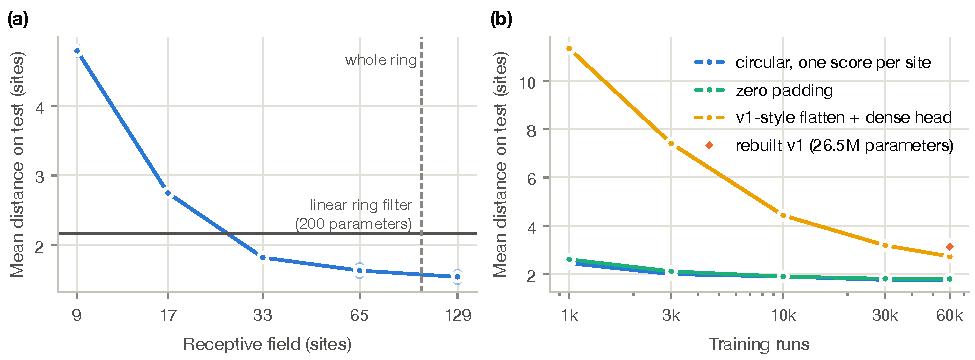
\includegraphics[width=\linewidth]{paper_fig4_ring.pdf}
  \caption{(a)~Mean test distance of a dilated circular CNN against its receptive field; the line is the 200-parameter linear ring filter. (b)~Mean test distance against the number of training runs for the two-branch network described in the text (shallow circular convolutions plus a global branch on the lowest ring modes) with one score per site, the same with zero padding, and with a v1-style flatten and dense head; the diamond is the rebuilt v1, trained on 60,000 runs. Zero padding costs far less here than in the final model (Table~\ref{tab:choices}), presumably because the global branch is periodic whatever the padding.}
  \label{fig:ring}
\end{figure}

The receptive field, the stretch of the ring that a pendulum's features see, matters most [Fig.~\ref{fig:ring}(a)]. In a circular CNN of four to seven layers with kernels of three sites, spreading the three sites further apart from layer to layer (dilation) widens the receptive field from 9 to 129 sites, and the mean distance falls from 4.79 to 1.54. A network that sees only nine pendulums is worse even than the linear ring filter, which sees the whole ring.

Our first design reached the whole ring differently. Since the linear growth stage multiplies each ring mode by its own factor, we combined a shallow local branch of circular convolutions with a global branch that keeps only the lowest ring modes and multiplies each by a learned complex matrix that mixes the channels, a generalization of the Floquet response and the form of Fourier neural operators \cite{li2021fourier}. The two branches together beat either alone, and the global branch saturates once it includes the unstable band, as expected. The deep whole-ring CNN does better still, however, and gains nothing from the global branch, presumably because deciding which of several growing humps wins is a nonlinear competition across the ring that no linear filter captures.

The ring's symmetry, in turn, saves data [Fig.~\ref{fig:ring}(b)]. A network that scores every site with the same filters needs to learn each pattern only once \cite{cohen2016group}; trained on 1,000 runs, the two-branch network with one score per site already beats its flatten-and-dense counterpart trained on 60,000.

Whether the frames still benefit from a recurrent layer turned out to be a closer question than we had expected. On the two-branch network, passing each pendulum's convolved frames through a small gated recurrent unit (GRU) \cite{cho2014learning} did help, lowering the mean distance from 1.75 with stacked frames to 1.59, although a small per-pendulum network without recurrence recovered part of this gain. In the whole-ring CNN, however, the advantage disappears: it scores 1.54 with stacked frames and 1.57 with the same GRU in front. On the validation pool the whole-ring CNN ties with the same network plus the global branch and with the two-branch network plus the GRU, and we chose the simplest of the three, the whole-ring CNN without recurrence.

One further idea did not pay off. Feeding the two-branch network the field evolved by the Floquet filter, which we expected to leave it only the nonlinear correction to learn, did not help even with only 3,000 training runs; the network learns the linear growth stage from the data alone. Nor does the network need to be large: versions of the two-branch network from 2,000 to 115,000 parameters all land within about a third of a site of each other, as one would expect if the answer lives in about ten numbers plus local texture. Other families of models seemed less suited and were not pursued: on a ring with nearest-neighbor coupling a graph network reduces to a one-dimensional convolution, a transformer over sites lacks the locality of the coupling, and reservoir computing \cite{Chaos_Ott_2017,PhysRevLett_Ott_2018} forecasts trajectories rather than a single outcome.

\subsection{Inputs and training}
\label{sec:inputs}

Energies were the natural input for v1, since the box-car analysis and the label of Ref.~\cite{mittal2026jand} are stated in terms of energy. They hold no information beyond the angles, velocities and coupling constants they are computed from, however, and at release, to first order in the offsets, $E_n(0)$ is a shifted, rescaled copy of $\theta_n(0)$. Energies are also expensive to measure, since velocities call for a gyroscope on every pendulum or noisy differencing of video frames, whereas one camera can track every angle. And $\theta_n(0)$ alone is the complete state (Sec.~\ref{sec:floquet}). We therefore expected the initial angles alone to match v1's inputs, and they did; frames of angles did better still, in screening runs of the whole-ring CNN (mean distances of 1.56 for ten angle frames, 1.66 for the initial angles alone, and 1.75 for v1's inputs) and on the cleaner labels of Sec.~\ref{sec:target}, since the later frames, though carrying no new information, make the same information easier to learn. Energies help when the observation starts at an unknown point in the swing, along which they barely change; angles then need about a full swing of frames to do as well.

For the loss, v1 used plain cross-entropy over the 100 sites, which counts a prediction one site off as just as wrong as one 50 sites off. Since neighboring sites are nearly equivalent at the level of the label (Sec.~\ref{sec:pools}), we expected soft labels \cite{szegedy2016rethinking}, here spread over the neighbors of the true site, to help, and they did, lowering the mean distance in screening runs from 1.75 to 1.58 and cutting the spread between seeds fourfold. Against our expectation, however, they also lower the share of exact hits (from 40\% to 28\% in full-length training). Regressing a position on the ring did worst, because it averages two competing humps into a site between them. Adding the expected ring distance to the loss did not help and made the model hedge at larger weights; we kept a small weight, with which the time head below was tested. Since the same growing modes set both when and where the energy localizes, we added a head that predicts the localization time, and it helped the site prediction slightly. The binary head of v1, which predicts whether a run localizes at all, adds nothing on undamped chains, where every run localizes. The optimizer, finally, is a question the physics does not answer. Against our guess that the learning-rate schedule would matter, every adaptive optimizer and schedule we tried landed within the spread between seeds; we kept AdamW \cite{loshchilov2019decoupled} with a cosine schedule \cite{loshchilov2017sgdr}, our default throughout, although Adam \cite{kingma2015adam} at a constant rate, as in the rebuilt v1, does about as well.

\subsection{The final model}
\label{sec:final}

The final model [Fig.~\ref{fig:schematic}(b)] feeds the ten angle frames of Sec.~\ref{sec:inputs}, taken over the observation window of v1, to the whole-ring CNN of Sec.~\ref{sec:arch}: seven circular convolutions of 32 channels with kernels of three sites, at dilations 1, 2, 4, 8, 16, 32 and 1 \cite{yu2016multiscale,oord2016wavenet}. A small head, the same at every pendulum, gives a score $s_n$ per site and the probability $p_n=e^{s_n}/\sum_{n'}e^{s_{n'}}$, and a second head, linear in the ring-averaged features, predicts the logarithm of the localization time $\tau_{\mathrm{loc}}$. With $y$ the true site, the loss is
\begin{equation}
\label{eq:loss}
\mathcal{L} = -\sum_n q_n\ln p_n + \lambda_d\sum_n p_n\, d(n,y) + \lambda_t\left(\hat\ell-\ell\right)^2,
\qquad q_n\propto\exp\!\left[-\frac{d(n,y)^2}{2\sigma^2}\right],
\end{equation}
that is, cross-entropy against soft labels of width $\sigma=1$ site, plus $\lambda_d=0.1$ times the expected ring distance, plus $\lambda_t=0.1$ times the squared error of the predicted log-time $\hat\ell$, where $\ell=(\ln\tau_{\mathrm{loc}}-\ln57)/0.2$. The model has 22,786 parameters, none of them tied to a particular pendulum, and trains in about six minutes on the same 60,000 runs as the rebuilt v1.

Table~\ref{tab:headline} compares it with v1 and the baselines. Against the rebuilt v1, v2 halves the mean distance, from 3.14 to 1.49, cuts the far misses from 5.7\% to 1.5\%, and raises the share within $\pm1$ from 60\% to 77\%. It does so with about a thousandth of the parameters and a quarter of the training time. Yet v2 does not reach the 94.4\% within $\pm1$ reported in Ref.~\cite{mittal2026jand}, a point we return to in Sec.~\ref{sec:repro}.

\begin{table}[t]
  \centering
  \caption{The design choices of v2, the physical reason for each, and the cost of reverting each toward v1's choice in the final model, which need not be its cost in v1 (three seeds each; test pool, first-crossing label). $\Delta$ is the change in mean distance against the final model's 1.49 (positive is worse), $\pm$ its standard error. $^*$The same seven layers without dilation, so that each pendulum sees 15 sites. $^\dagger$From the architecture comparison with v1's inputs: adding a per-pendulum GRU in front of the whole-ring CNN (1.57 against 1.54; within $\pm1$, 73.1\% against 75.6\%).}
  \label{tab:choices}
  \footnotesize
  \setlength{\tabcolsep}{3.5pt}
  \renewcommand{\arraystretch}{1.15}
  \begin{tabular}{@{}>{\raggedright}p{2.1cm}>{\raggedright}p{2.75cm}>{\raggedright}p{4.1cm}>{\raggedright}p{2.75cm}rr@{}}
    \toprule
    Choice & v2 & Physical reason & v1 & $\Delta$ if reverted & $\pm1$ (\%) \tabularnewline
    \midrule
    Receptive field & whole ring (129~sites) & the growing modes are the longest waves & 9 sites per feature; whole ring only via the LSTM & $+1.10\pm0.01^*$ & 59.0 \tabularnewline
    Boundary & circular padding & the ring has no ends & zero padding & $+0.93\pm0.04$ & 66.7 \tabularnewline
    Output & one score per site & the dynamics are the same at every pendulum & flatten and dense layers & $+0.31\pm0.02$ & 72.0 \tabularnewline
    Frames & frames stacked as channels & little growth or travel within the window & per-frame convolutions and a BiLSTM & $+0.03\pm0.03^\dagger$ & 73.1$^\dagger$ \tabularnewline
    Loss & soft labels, distance and time terms & neighboring sites are nearly equivalent & cross-entropy & $+0.08\pm0.02$ & 64.3 \tabularnewline
    Inputs & angle frames & a camera measures angles; $\theta_n(0)$ is the full state & energies and $\theta_n(0)$ & $+0.02\pm0.02$ & 76.4 \tabularnewline
    Optimizer & AdamW, cosine schedule & none; the physics is silent here & Adam, default settings & $+0.07\pm0.04$ & 75.8 \tabularnewline
    \midrule
    \multicolumn{4}{@{}l}{Final model} & 1.49 & 77.2 \tabularnewline
    \bottomrule
  \end{tabular}
\end{table}

We then retrained the final model with one choice reverted at a time, and Table~\ref{tab:choices} pairs each choice with the reason it was made. The three architectural choices that the ring's physics dictates matter most. Seeing the whole ring is worth 1.1 sites, circular padding 0.9, and one score per site 0.3, the last while cutting the model's parameters tenfold. Once the architecture is right, v1's inputs and optimizer cost little. The loss matters mainly for the share within $\pm1$: with plain cross-entropy that share falls from 77\% to 64\%, for a reason we shall see in Sec.~\ref{sec:target}.

The network is also economical with data: trained on only 1,000 runs, v2 already beats the rebuilt v1 trained on 60,000 (2.42 against 3.14). Nor does it need much explicit regularization. Because no parameter is tied to a particular pendulum, it does nearly as well on the test pool as on its training runs (1.49 against 1.35) with no dropout \cite{srivastava2014dropout} and only a small weight decay, whereas the rebuilt v1 overfits despite dropout and early stopping (3.00 against 1.62 for one seed). Where v2 does overfit, with little data, dropout makes it worse and weight decay up to $10^{-1}$ changes nothing. What helps is adding the mirror images of the training runs, the one symmetry of the ring that the network does not build in: they are worth about twice the data, and they slow the overfitting enough for a weight decay of 1 to act.

Finally, is the localization time worth predicting for its own sake, or does it merely follow the parameters of the run, as we suspected? The time head predicts it to a median error of 1.5\%, but most of the timing is a trend in the amplitude, which alone predicts it to 5.0\%; the remaining gain is only about two time units. As the amplitude dependence of the localization time in Ref.~\cite{mittal2026jand} already suggested, \emph{when} the energy localizes is largely set by the amplitude, whereas \emph{where} it localizes is the real prediction problem.

\subsection{What to predict}
\label{sec:target}

Most of v2's remaining error on the first-crossing label turns out to belong to the label. Within one swing, the energy of a forming hotspot moves back and forth between a pendulum's motion and the springs on either side of it, so which pendulum first crosses 10\% depends on the moment in the swing at which the threshold is passed. To remove this exchange, we define a \emph{swing-averaged label}: we split each spring's energy evenly between the two pendulums it joins, which gives a symmetric site energy $E^{\mathrm{s}}_n$, and average it over the last 16 samples, about one swing,
\begin{equation}
\label{eq:avg}
\bar E_n(\tau_k) = \frac{1}{16}\sum_{j=0}^{15} E^{\mathrm{s}}_n(\tau_{k-j}) ;
\end{equation}
the label is the top site at the first sample at which $\max_n\bar E_n>0.1\,\Etot$. The two labels agree exactly in only a third of the test runs, the averaged one usually sitting one to three sites to the left [Fig.~\ref{fig:jitter}(a)]. The jitter shows up in the errors, too. Trained with plain cross-entropy, v2 misses by two sites more often than by one, and half of those two-site misses sit exactly on the swing-averaged position [Fig.~\ref{fig:jitter}(b)]. Soft labels hedge between the two candidate sites, which is why they raise the share within $\pm1$ so much.

\begin{figure}[t]
  \centering
  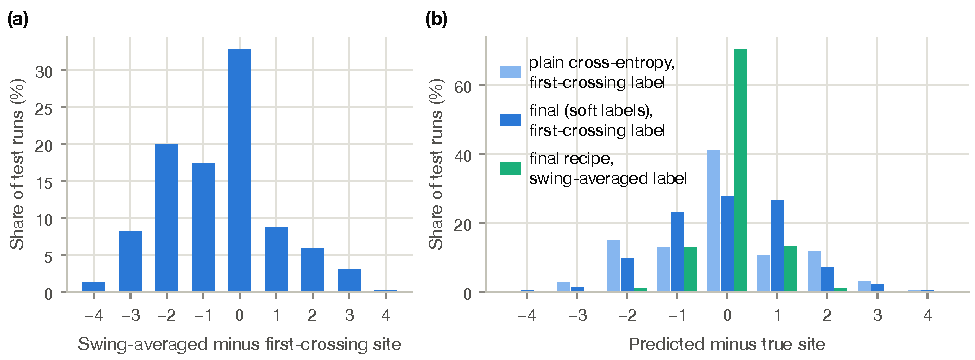
\includegraphics[width=\linewidth]{paper_fig5_jitter.pdf}
  \caption{(a)~Swing-averaged site minus first-crossing site on the test pool. (b)~Prediction errors of v2 trained with plain cross-entropy and of the final model (soft labels), both on the first-crossing label, and of the same recipe trained and scored on the swing-averaged label.}
  \label{fig:jitter}
\end{figure}

This raises a more basic question: is a single pendulum the right target at all? When the first-crossing label fires, the top pendulum holds 10.3\% of the energy at that instant but only 5.5\% averaged over a swing, and the swing-averaged hump is about eight pendulums wide at half height. The 10\% on a single pendulum is thus the instantaneous peak of a breathing hump. The hump stays in place for about a swing after it forms, then drifts. In about one run in six a rival hump at least five sites away holds at least half as much energy, so that any single-site answer is a guess between two places. We therefore also define the event at the scale of the hump. The \emph{hump label} fires at the first sample at which
\begin{equation}
\label{eq:hump}
\max_n H_n > 0.15\,\Etot , \qquad H_n = \bar E_{n-1} + \bar E_n + \bar E_{n+1} ,
\end{equation}
and names the center of that three-pendulum window. Its threshold of 15\% was chosen so that it fires together with the first-crossing label, at a median of 54.5 against 55 time units, whereas the swing-averaged label fires about five time units later; below, we replace this threshold with a physical event.

\begin{table}[t]
  \centering
  \caption{The same recipe trained and scored on each label (test pool; seeds in brackets). Accuracies in \%.}
  \label{tab:labels}
  \small
  \begin{tabular}{@{}llrrrr@{}}
    \toprule
    Model & Label [seeds] & Mean dist. & Exact & $\pm1$ & $>10$ off \\
    \midrule
    v2 & First crossing [5] & 1.49 & 27.7 & 77.2 & 1.5 \\
    v2 & Swing-averaged [3] & 0.58 & 70.5 & 96.4 & 0.7 \\
    v2 & \textbf{Hump [3]} & \textbf{0.27} & \textbf{84.7} & \textbf{99.4} & \textbf{0.4} \\
    \midrule
    v1 rebuilt & First crossing [2] & 3.14 & 22.5 & 60.4 & 5.7 \\
    v1 rebuilt & Swing-averaged [2] & 2.25 & 42.0 & 83.6 & 4.4 \\
    \bottomrule
  \end{tabular}
\end{table}

We trained and scored the same recipe on each label (Table~\ref{tab:labels}). On the swing-averaged label v2 reaches a mean distance of 0.58, with 96.4\% within $\pm1$, and on the hump label 0.27, with 99.4\%. Sharing the springs evenly without averaging over a swing does not help, so the jitter comes from the energy moving within each swing, not from how the spring energy is assigned. The hump label's further gain in mean distance over the swing-averaged label comes about equally from being read when the hump forms and from naming the center of a three-pendulum window rather than the top pendulum. The first 4.5 time units thus decide where the hump forms: even the model trained on the first-crossing label is within $\pm1$ of the hump label in 91\% of runs.

Since every design choice of Secs.~\ref{sec:arch} and \ref{sec:inputs} was made on the jittery first-crossing label, we repeated the key ones on the cleaner labels. They hold, and seeing the whole ring matters even more: with a four-layer stack that sees only 17 sites the mean distance triples on the swing-averaged label and grows more than fivefold on the hump label, against 1.6-fold on the first-crossing label. Soft labels, by contrast, stop mattering, and on the hump label hard labels do slightly better; on a label that does not jitter, the hedge only blurs the answer. The target is therefore best framed as the center of the hump when it forms, with a probability over all pendulums as output.

This leaves the threshold itself. The 10\% threshold of Ref.~\cite{mittal2026jand} was set ``somewhat arbitrarily''. A scale with physical meaning is the separatrix energy $E_{\mathrm{sep}}=2$, the on-site energy of a pendulum held at the top in Eq.~(\ref{eq:energy}). With $\Etot\approx118$ it is 1.7\% of the total, so the 10\% threshold asks one pendulum for about six times $E_{\mathrm{sep}}$. An event that needs no threshold at all is the first pendulum to swing past the top, $|\theta_n|>\pi$, where its libration turns into rotation; it happens at a median of $\tau=50$, close to the first crossing of 3--4\% of the total energy (median lags of $-1.5$ and $+1.5$ time units). We recomputed the first-crossing label at 3--15\% of the total energy and trained the final recipe on each, with three seeds (Fig.~\ref{fig:threshold}). Up to 5\% the label fires a median of at most two time units from the first pendulum past the top and names it within $\pm1$ in 99\% of runs, and v2 places 99.1--99.4\% of runs within $\pm1$, as on the hump label. The most accurate threshold is 4\%, about 2.4\,$E_{\mathrm{sep}}$, with a mean distance of 0.34. Beyond 5\% the label fires later, while energy passes to the neighbors, and accuracy falls to a minimum of 77.1\% at the 10\% of Ref.~\cite{mittal2026jand}, recovering partly at 15\% as one pendulum comes to dominate the hump. The training-free Floquet filter and the rebuilt v1 follow the same curve, with 72.6\% and 88.5\% at 4\% against 52.0\% and 60.1\% at 10\%. Across the thresholds, v2's accuracy rises and falls with the share of runs whose label lies within $\pm1$ of the hump center (Spearman $\rho=0.99$) and with the Floquet filter's accuracy ($\rho=0.93$): the label is learnable exactly where the physics pins it. Labeling the first pendulum past the top directly gives 98.9\%. The best threshold for learning is thus not arbitrary; it marks the first pendulum going over the top. A threshold on the share of the total energy also means something different on rings of other sizes, since the share held by one pendulum scales as $1/N$ (Sec.~\ref{sec:realchain}). Its role here is therefore to explain, and we keep 10\% only for the comparisons with v1.

\begin{figure}[t]
  \centering
  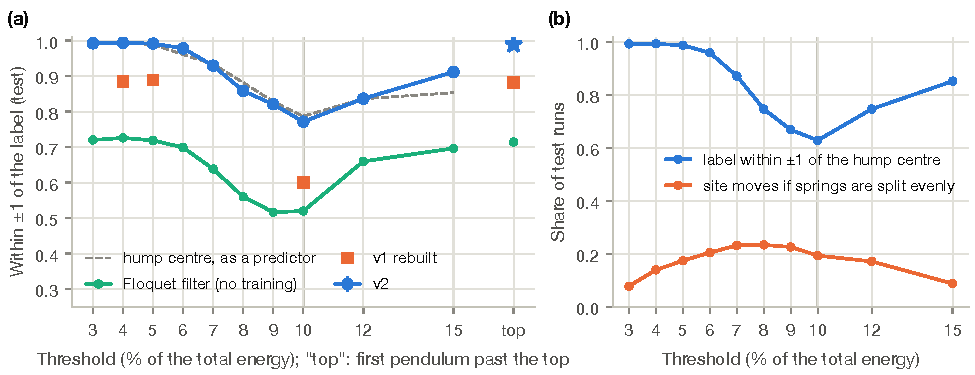
\includegraphics[width=\linewidth]{paper_fig7_threshold.pdf}
  \caption{(a)~Accuracy within $\pm1$ of the first-crossing label on the test pool against the threshold, for v2 (three seeds; mean and standard deviation), the rebuilt v1 (two trained seeds), the Floquet filter, and the hump center used as a predictor; ``top'' labels the first pendulum past the top. (b)~Share of test runs whose label lies within $\pm1$ of the hump center, and whose labeled site changes if each spring's energy is split evenly between neighbors.}
  \label{fig:threshold}
\end{figure}
We therefore let the event itself time the hump label. At the moment the first pendulum passes the top, we average the symmetric site energy over the swing centered on that moment and name the center of the three neighboring pendulums that hold the most energy. This \emph{event-timed hump label} has no energy threshold: it fires at a physical event, its window is one swing, and three pendulums is the narrowest window that finds the center of a flat-topped hump. It lies within $\pm1$ of the hump label of Eq.~(\ref{eq:hump}) in 99.6\% of test runs, and v2 places 99.4\% of runs within $\pm1$ of it, as on that label, with a mean distance of 0.28 against 0.27 (Table~\ref{tab:labels}). Its remaining choices hardly matter: windows of three to seven pendulums and thresholds of the hump label between 10\% and 20\% change v2's accuracy by at most 0.2 points, except for three pendulums at 20\% (98.0\%), which fires seven time units after the event, when rival humps have had longer to compete. Wider windows score better on their own labels but locate the hump no better against a common reference; their center is a smoother target, not a sharper answer. Following a rule fixed before these runs, the event-timed hump label is our recommended target, and since it agrees so closely with that of Eq.~(\ref{eq:hump}), the results obtained on the latter carry over.

\subsection{Toward a real chain}
\label{sec:realchain}

A real chain will be observed with noisy sensors, and its parameters will be known only approximately. Since an error of $10^{-3}$~rad in the initial state already moves a quarter of the labels (Sec.~\ref{sec:physics}), let us first look at sensor noise. We trained the network on camera-like data, eight angle frames 0.5 time units apart with Gaussian noise on every pendulum and frame, starting the observation at $\tau=0$, 10, 20 or 30. Watching from release, the camera does well up to about $10^{-3}$~rad and degrades beyond. Interestingly, noise first causes far misses: the share within $\pm1$ hardly changes at first, while the share of far misses triples. Noise picks the wrong hump before it blurs the right one.

\begin{figure}[t]
  \centering
  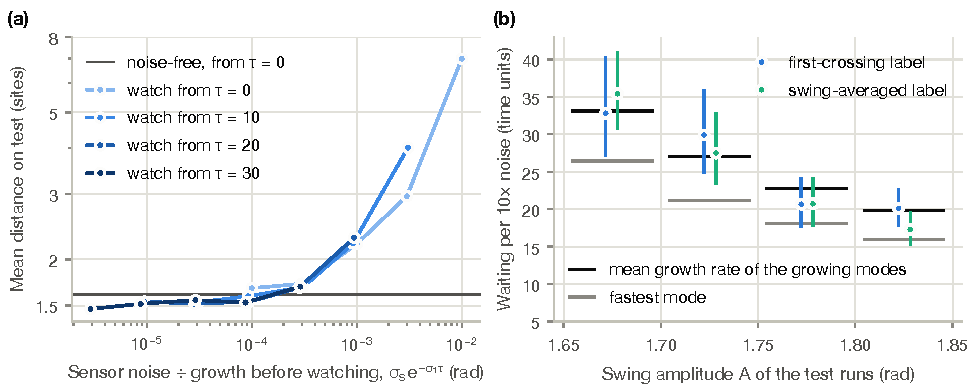
\includegraphics[width=\linewidth]{paper_fig6_noise.pdf}
  \caption{Waiting divides the sensor noise by the growth of the unstable modes. (a)~Mean distance of the camera setup (first-crossing label; one seed per cell) against the sensor noise $\sigma_s$ divided by the growth of the fastest mode since release, for observations starting at $\tau=0$, 10, 20 and 30; the horizontal line is the noise-free error from release. (b)~Waiting per tenfold noise for the camera in four amplitude bins, on the first-crossing and swing-averaged labels (dots, fits; bars, 95\% intervals), against the predictions from the mean growth rate of the growing modes and from the fastest mode.}
  \label{fig:noise}
\end{figure}

Waiting helps, because the growing modes rise above the sensor noise while the noise does not grow. If the fastest mode alone set the pace, each tenfold increase in sensor noise would cost $\ln10/\sigma_1$, about 20 time units of waiting, and this was our initial prediction. Figure~\ref{fig:noise} shows that waiting pays off more slowly. The camera's error depends on the noise and the start time essentially through the noise relative to the grown signal [Fig.~\ref{fig:noise}(a)], but each tenfold increase in noise costs about 25 time units, close to what the mean growth rate of the growing modes gives rather than the fastest one. A likely reason is that white noise enters every ring mode equally, while the site depends on all the growing modes, each of which rises above the noise at its own rate. We found this rate on the first-crossing label and wrote it down as a prediction for the swing-averaged label before any later-start run on that label had finished: 24.8 time units predicted, 25.5 measured. Split by amplitude, the waiting cost falls as the growth rates rise [Fig.~\ref{fig:noise}(b)]. In practice, with v2's ten frames, a camera ten times coarser than $10^{-3}$~rad catches up with a precise one if it starts watching about 25 time units later, which for 20~cm pendulums still leaves about 3.6~s of warning.

Fewer sensors cost less than one might fear. Tracking every second pendulum costs nothing, with or without noise, and every fourth costs little without noise. Every eighth fails, however. Its 13 sensors satisfy the Nyquist criterion for the five growing modes, which we had expected to suffice, but at release the stable modes hold about 90\% of the perturbation, and on 13 sensors they alias onto the wavenumbers of the growing ones. Putting this together, one camera tracking every second pendulum to $10^{-3}$~rad, with v2's ten frames from release, scores a mean distance of 1.93 on the first-crossing label, well ahead of the rebuilt v1 with perfect data (3.14), and locates the forming hump within $\pm1$ in 96.8\% of runs. For 20~cm pendulums, $10^{-3}$~rad is 0.2~mm at the bob; we estimate, but have not tested, that one camera at 30--60 frames per second tracking markers on the bobs can reach it.

\begin{table}[t]
  \centering
  \caption{Models trained on the nominal chain, tested without retraining on shifted chains (pools of 5,000 runs simulated with their own true parameters) and with sensor noise added to the nominal test pool. Mean distance on the first-crossing label, over the runs that localize by $\tau=150$: nearly all, except at $\htl$ $+10\%$, where 80\% do. The last column describes the growth spectrum at $A=1.75$.}
  \label{tab:robust}
  \small
  \begin{tabular}{@{}lrrl@{}}
    \toprule
    Test condition & v1 rebuilt & v2 & Growth spectrum at $A=1.75$ \\
    \midrule
    Nominal chain & 3.14 & 1.49 & 5 growing modes, $\sigma_1=0.1185$ \\
    Neighbor coupling $\gt$ $\pm10\%$ & 3.26 / 3.39 & 1.97 / 1.97 & essentially unchanged \\
    Twice the initial spread & 3.62 & 1.96 & unchanged \\
    Global coupling $\htl$ $-10\%$ & 4.36 & 4.25 & $\sigma_1$ $+21\%$; 6 modes grow; $A_c=1.48$ \\
    Global coupling $\htl$ $+10\%$ & 5.91 & 5.53 & $\sigma_1$ $-33\%$; 3 modes grow; $A_c=1.68$ \\
    $N=80$ / $150$ pendulums & n/a & 1.31 / 6.32 & 4 / 8 modes grow \\
    One pendulum 2~mm longer & 18.9 & 22.9 & the impurity attracts the site \\
    Sensor noise $10^{-3}$~rad & 6.24 & 2.26 & \\
    \bottomrule
  \end{tabular}
\end{table}

The parameters of a real chain will also be off. We applied both networks, trained on the nominal chain, to shifted ones (Table~\ref{tab:robust}), and the damage again follows the Floquet spectrum. Errors that leave the spectrum essentially unchanged, in the neighbor coupling or the initial spread, cost v2 about half a site. A 10\% error in the global coupling, by contrast, changes how fast and how many modes grow, and both networks fall to 4--6 sites, which erases most of v2's lead; $\htl$ must therefore be known to a few percent, or the model trained over a range of it. Because v2 scores every site with the same filters, it also runs on rings of other sizes, which v1 cannot, although it degrades at 150 pendulums, for a reason we return to below. As found in Ref.~\cite{mittal2026jand}, an impurity strongly attracts the localization. A single pendulum about 2~mm longer, whose restoring term in Eq.~(\ref{eq:eom}) is therefore 1\% weaker, pins the site within $\pm3$ of it in 92\% of runs and defeats both networks, which have never seen such a cue. Retrained on chains with one random pendulum up to 2\% weaker, v2 finds it from the motion alone, since a longer pendulum swings slightly slower, and reaches a mean distance of 1.06.

These tests applied a network to conditions it had not seen. To find out what a network must be trained on, we also trained the recipe on the event-timed hump label at fixed amplitudes, at other offset sizes and on rings of other sizes (Fig.~\ref{fig:training}). A network trained at a single amplitude places 99.5--99.7\% of runs within $\pm1$ from 1.65 to 1.95, and one trained over the whole interval does as well to within 0.6 points, so a narrower range of amplitudes, which one might expect to make the problem easier, makes little difference. Only at the threshold, $A=1.60$, where the outcome changes steeply with the amplitude, does the network trained there gain (98.7\% against 85.8\%). Nor does a network extrapolate. The one trained on 1.65--1.85 places 90\% of runs within $\pm1$ at 1.90, 50\% at 1.95 and 25\% at 1.60, and the one trained at the stated offsets 93\% at twice the offsets and 65\% at four times, where networks trained at those sizes reach 99.3\% and 99.1\%.

A longer ring holds more growing modes, about $N/20$ at $A=1.75$, at the same rates, so the ring size sets how many modes compete. On rings of 50 to 400 pendulums, with two more dilated layers (dilations 64 and 128) so that every pendulum sees a stretch of 513, the number of growing modes rises from two to 22 and the share of runs with a rival hump at least half as large from 2.4\% to 71\%, yet the share within $\pm1$ falls only from 99.9\% to 98.8\%. This is consistent with the hump forming where the growing band focuses the energy, as in the modulational instability of discrete lattices \cite{kivshar1992modulational}, however many modes compete. Networks carry over from longer rings to shorter ones, those trained on 200 and 400 pendulums keeping 98.9\% and 95.3\% at $N=100$, but not the reverse: the network trained at $N=100$ places only 30\% of runs within $\pm1$ on a ring of 200, although it sees the whole ring, whereas the standard network, which sees 129 pendulums, keeps 92\%. Our expectation that seeing the whole ring would suffice was thus wrong. A likely reason is that on a long ring the growing modes form a nearly continuous band and the hump forms by a local process whose scale does not depend on $N$, whereas on the 100-pendulum ring a network can rely on its five particular global modes. On rings of other sizes, a threshold on the share of the total energy also loses its meaning: at $N=400$, 10\% is 40 times one pendulum's share, and the first-crossing label had fired in only 2.9\% of test runs when the event-timed label was complete. A model for a real chain must thus be trained over the amplitudes at which the chain will be released, at its release scatter, and on a ring at least as long.

\begin{figure}[t]
  \centering
  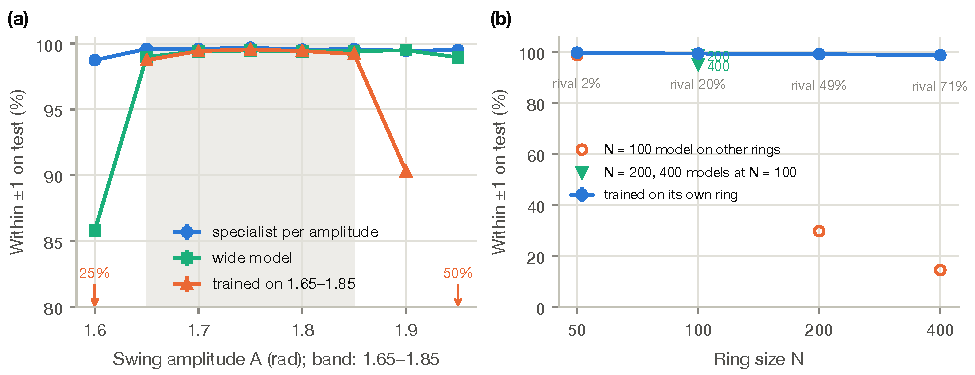
\includegraphics[width=\linewidth]{paper_fig_training.pdf}
  \caption{What a network must be trained on (event-timed hump label, test pools, three seeds). (a)~Accuracy within $\pm1$ at fixed amplitudes for networks trained at that amplitude, over 1.60--1.95, and over 1.65--1.85 (band); arrows mark values below the axis. (b)~Networks trained on rings of 50--400 pendulums, scored on their own ring (labels: share of runs with a rival hump at least half as large), the network trained at $N=100$ scored on the other rings, and those trained at $N=200$ and 400 scored at $N=100$.}
  \label{fig:training}
\end{figure}

Real pendulums also lose energy, and the missing damping was the main gap we saw between our simulations and a real chain. With linear damping the uniform swing decays toward the threshold $A_c$, so a run localizes only if its perturbation has grown enough before then: at a quality factor $Q\ge1{,}000$ almost every run still localizes, at $Q\approx330$ only 71\% do, and at $Q=100$ none do, and integrating the Floquet growth rate along the decaying swing predicts the delay. Retrained on damped chains, v2 even improves with damping, to 0.84 at $Q\approx330$ on the runs that localize, presumably because near threshold fewer and longer modes grow and the site depends less on local detail; these are not simply the easy runs, since without damping v2 does worse on them than on the rest. Here v1's binary ``localizes'' head (Sec.~\ref{sec:inputs}) earns its place: from the first 4.5 time units it tells whether a run will localize at all, correctly in 99.5\% of damped runs.

% ===========================================================================
\section{Reproduction of the earlier network}
\label{sec:repro}

% TODO-AUTHOR-REVIEW: This section is still being discussed with the corresponding author of
% Ref. [mittal2026jand] (wording of the discrepancy; access to the original training notebook).
% Keep it neutral and within what REPORT.md (Sec. 2) supports. Do not post before agreed.
\authorreview{This section is under discussion with the corresponding author of Ref.~\cite{mittal2026jand}, including how to word the discrepancy and whether the original training code can be recovered. It states only what the rebuild shows; do not post before the wording is agreed.}

The training code and dataset of Ref.~\cite{mittal2026jand} were not available for this study, so we rebuilt the CNN-BiLSTM from the description in Sec.~2.3 and the Appendix of that paper, keeping the defaults of the TensorFlow (Keras) layers it names. Its data come from a simulator that gives the same localization site and time as the simulation code of Ref.~\cite{mittal2026jand} on 1,000 of 1,000 test runs, and the only deliberate change is that the input scaler is fitted on the training pool alone. The rebuild does not reproduce the accuracy reported in Ref.~\cite{mittal2026jand}: two seeds reach 61.7\% and 59.1\% within $\pm1$, against the published 94.4\%, and mean distances of 3.00 and 3.27, against 1.44; a third seed never trained.

The gap appears to lie in the settings rather than in the network. The first-crossing label at 10\% of the total energy fires about five time units after the first pendulum swings past the top, when energy is already passing to its neighbors, which is why it jitters (Sec.~\ref{sec:target}). Retrained on first-crossing labels at lower thresholds, and otherwise unchanged, the rebuild recovers most of the published accuracy (Table~\ref{tab:repro}). The offsets probably differed too. The original data-generation code sets a noise level of 0.025, and the simulation code of Ref.~\cite{mittal2026jand} applies a noise level $s$ as offsets $s\,(U-\tfrac12)$; read this way, the training data had offsets $\eta_n\sim\mathcal{U}(-0.0125,0.0125)$, half those stated. At a 4\% threshold and these offsets the rebuild reaches 92.5\% within $\pm1$ and a mean distance of 1.69, against the published 94.4\% and 1.44, although at such small offsets most seeds never leave the loss of a uniform guess (App.~\ref{app:training}). As far as we can reconstruct them, the accuracies published in Ref.~\cite{mittal2026jand} were therefore obtained with an effective threshold of about 4\% of the total energy and offsets of $\pm0.0125$, rather than the 10\% and $\pm0.025$ stated there; we could not check these settings against the original training code. Every comparison with v1 in this paper nevertheless uses the stated settings, at which the rebuild reaches 60.4\% within $\pm1$ and v2 77.2\% (Table~\ref{tab:headline}). At the reconstructed settings v2 reaches 99.4\%. The few points where the published description and the simulation code of Ref.~\cite{mittal2026jand} differ otherwise, such as the time axes of its figures, which count samples of 0.5 time units, are listed in the report that accompanies our code.

\begin{table}[t]
  \centering
  \caption{The rebuilt v1 and v2 at the settings stated in Ref.~\cite{mittal2026jand} and at lower thresholds, on the 20,000-run test pool (trained seeds in brackets). At offsets of $\pm0.0125$, runs that have not localized by $\tau=100$ are left out, as in the original data. The runs of Table~\ref{tab:headline} give 3.14 and 60.4 (v1) and 1.49 and 77.2 (v2) at the stated settings. Distances in sites, accuracies in \%.}
  \label{tab:repro}
  \small
  \begin{tabular}{@{}llrrrr@{}}
    \toprule
    & & \multicolumn{2}{c}{v1 rebuilt} & \multicolumn{2}{c}{v2 [3]} \\
    \cmidrule(lr){3-4}\cmidrule(l){5-6}
    Threshold & Offsets & Mean dist. & $\pm1$ & Mean dist. & $\pm1$ \\
    \midrule
    10\% (stated) & $\pm0.025$ (stated) & 3.07 [2] & 60.1 & 1.49 & 77.1 \\
    5\% & $\pm0.025$ & 2.12 [2] & 88.9 & 0.38 & 99.1 \\
    4\% & $\pm0.025$ & 2.16 [2] & 88.5 & 0.34 & 99.4 \\
    4\% & $\pm0.0125$ & 1.69 [1] & 92.5 & 0.32 & 99.4 \\
    \midrule
    \multicolumn{2}{@{}l}{As published \cite{mittal2026jand}} & 1.44 & 94.4 & & \\
    \bottomrule
  \end{tabular}
\end{table}

% ===========================================================================
\section{Conclusions}
\label{sec:conclusions}

In this study we revisited the prediction of where a noise-seeded type-III instability localizes energy in a sine-Gordon pendulum ring, starting this time from the physics of the instability rather than from the data. The Floquet growth spectrum of the uniform swing explains much of what was found empirically before. Only a handful of the longest ring modes grow, and this sets the optimal width of the box-car smoothing of Ref.~\cite{mittal2026jand}. The outcome is deterministic, so prediction is limited by how precisely the initial state is measured rather than by chaos, and the coarse answer lives in the amplitudes and phases of the few growing modes. The spectrum also sets the clock: localization takes 5--6 $e$-foldings of the fastest mode at any amplitude, each halving of the release scatter adds about $\ln2/\sigma_1$, and linear theory locates the site the better, the smaller the offsets are compared with the distance above threshold.

The same spectrum guided the design of the neural predictor. Since little grows or travels during the observation window while the growing modes span the whole ring, the network must see the whole ring, and once it does, the recurrent layer of v1 is not needed. Since the dynamics are the same at every pendulum, the network should apply the same filters everywhere and score every pendulum the same way. A circular CNN built on these principles, with a thousandth of the parameters, halves the error of our rebuild of the CNN-BiLSTM, beats it with 60 times less training data, and barely overfits. To answer the question left open in Ref.~\cite{mittal2026jand}, the features that decide the localization site are largely the projections of the early state onto the few growing long waves, with local detail deciding the last site or two.

The target deserves as much care as the model. The first pendulum to hold 10\% of the energy is the instantaneous peak of a breathing hump about eight pendulums wide, and most of the remaining error on that label is its own jitter; defined at the scale of the hump, the event fires just as early and is located within $\pm1$ in 99.4\% of runs. The threshold need not be arbitrary either: the first crossing of about 4\% of the energy marks the first pendulum to swing over the top and is predicted as well as the hump, whereas the 10\% of Ref.~\cite{mittal2026jand} lies near the worst choice. Timing the hump by that event leaves the target without any energy threshold, at no cost in accuracy. For a real chain, sensor noise can be traded against warning time at a cost set by the mean growth rate of the unstable modes, and in simulation one camera tracking every second pendulum already beats the rebuilt v1 with perfect data. A network must, however, be trained over the amplitudes and the release scatter of the chain, on a ring at least as long, since it does not extrapolate in amplitude or offset size and carries over only from longer rings to shorter ones.

These conclusions have limits. The comparison with v1 is against a rebuild, which reaches the published accuracy only at settings we reconstructed rather than read from the original code; if the rebuild differs from the original pipeline in another way that matters, the true gap could be smaller than reported here, although the physics baselines do not depend on the rebuild and v2 beats them too. Damping was simulated as linear, sensor noise as white, and impurities as a single lengthened pendulum, whereas a real chain will have small differences at every pendulum and correlated measurement errors. Testing the recommended setup on a bench-top chain is the natural next step.

% ===========================================================================
\section*{Data and code availability}

% TODO-AUTHORS: add a version tag or DOI (e.g. a Zenodo archive) when posting.
The simulator, data-generation scripts, training code, run logs and figure scripts used in this study are available at \url{https://github.com/adrian0729/sineGordonLocalization}, together with a report that gives the full set of ablations, including those summarized only briefly here.


% ===========================================================================
\appendix

\section{Training details}
\label{app:training}

\textit{v1, rebuilt.} Built as described in Sec.~\ref{sec:predictors}, with the defaults of the TensorFlow (Keras) layers named in Ref.~\cite{mittal2026jand} (26,499,205 parameters; Adam at a learning rate of $10^{-3}$, batch size 64, early stopping on the validation loss); training takes about 23 minutes. Some seeds never leave the loss of a uniform guess, $\ln100$, and these were repeated with another seed and are not scored: one of three at the stated settings, one of nine in the threshold study at the stated offsets, and 11 of 14 at offsets of $\pm0.0125$, presumably because the deviations that locate the hotspot are then smaller against the spread of amplitudes.

\textit{v2.} Hidden activations are GELUs \cite{hendrycks2016gelu}, and the per-site head is a circular convolution of kernel 3, a GELU and a $1\times1$ convolution. Training uses AdamW (learning rate $3\times10^{-3}$, weight decay $10^{-4}$) with a cosine decay and 3\% warmup, batch size 256, for 7,050 steps (30 epochs of 60,000 runs), keeping the checkpoint with the lowest validation mean distance, evaluated every 235 steps on 5,000 validation runs. The architecture comparison used the same budget. Screening runs had 15 epochs and three seeds (two for an unknown start, one per cell of the noise and sensor grids), so differences below about 0.1 sites there are within noise. The mirror image of a run maps pendulum $n$ to $N-1-n$, and its first-crossing label is the mirror image of the label computed with left-hand springs. Damping adds a term $-\gamma\dot\theta_n$ to Eq.~(\ref{eq:eom}), so that a free pendulum has quality factor $Q=1/\gamma$; every threshold is then a fraction of the energy the chain still holds.

\bibliographystyle{unsrtnat}
\bibliography{refs}

\end{document}
